% !TEX program = xelatex
\documentclass[11pt,a4paper,twoside]{article}
\usepackage[a4paper,top=2.1cm,bottom=2.6cm,inner=2.2cm,outer=2.2cm,footskip=1.3cm]{geometry}
\usepackage{fontspec}
\setmainfont{texgyrepagella}[Extension=.otf,UprightFont=*-regular,BoldFont=*-bold,ItalicFont=*-italic,BoldItalicFont=*-bolditalic,Path=/usr/share/texmf/fonts/opentype/public/tex-gyre/]
\setsansfont{FiraSans}[UprightFont=*-Regular,BoldFont=*-SemiBold,ItalicFont=*-Italic,Extension=.ttf,
  Path=/usr/share/fonts/truetype/google-fonts/ofl/firasans/]
\newfontfamily\heavy{FiraSans}[UprightFont=*-Bold,Extension=.ttf,Path=/usr/share/fonts/truetype/google-fonts/ofl/firasans/]
\usepackage{amssymb}
\usepackage{xcolor,tikz,tcolorbox,enumitem,multicol,fancyhdr,ragged2e,array,calc,pifont,hyperref}
\usetikzlibrary{shapes.geometric,calc,shadings}
\tcbuselibrary{skins,breakable}
\hypersetup{hidelinks,pdftitle={Własności liczb naturalnych – karty pracy},pdfauthor={karty pracy}}
\definecolor{pom}{HTML}{EE7F22}\definecolor{pomd}{HTML}{C85F0E}\definecolor{pomj}{HTML}{F8B25A}
\definecolor{piasek}{HTML}{F7DCAE}\definecolor{krem}{HTML}{FFF1DC}\definecolor{szary}{HTML}{8B8F99}
\definecolor{kratka}{HTML}{BFD3E6}\definecolor{ziel}{HTML}{5FA83A}\definecolor{czer}{HTML}{E0533D}
\definecolor{nieb}{HTML}{2F8FD1}\definecolor{fiol}{HTML}{8A5CC4}\definecolor{zolty}{HTML}{FFD54F}
\definecolor{tlozolte}{HTML}{FFE16B}
\setlength{\parindent}{0pt}\setlength{\parskip}{4pt}
\raggedright\emergencystretch=3em
\makeatletter\g@addto@macro\@parboxrestore{\raggedright}\makeatother
\hyphenpenalty=10000\exhyphenpenalty=10000
\setlist{nosep,leftmargin=*}

% ---------------- page style ----------------
\newcommand\stopka{}
\pagestyle{fancy}\fancyhf{}\renewcommand{\headrulewidth}{0pt}
\fancyfoot[C]{\begin{tikzpicture}[remember picture,overlay]
  \fill[piasek] (current page.south west) rectangle ([yshift=1.6cm]current page.south east);
  \ifodd\value{page}
    \node[anchor=west,font=\sffamily\small,text=pomd!70!black] at ([xshift=2.2cm,yshift=.8cm]current page.south west) {\stopka};
    \node[anchor=east,font=\sffamily,text=black] at ([xshift=-2.2cm,yshift=.8cm]current page.south east) {\thepage};
  \else
    \node[anchor=west,font=\sffamily,text=black] at ([xshift=2.2cm,yshift=.8cm]current page.south west) {\thepage};
    \node[anchor=east,font=\sffamily\small,text=pomd!70!black] at ([xshift=-2.2cm,yshift=.8cm]current page.south east) {WŁASNOŚCI LICZB NATURALNYCH};
  \fi
\end{tikzpicture}}

\newcommand\lekcja[2]{\clearpage\renewcommand\stopka{#1}%
\begin{tikzpicture}[remember picture,overlay]
  \shade[left color=pomj,right color=pomd,middle color=pom] ([yshift=-1.2cm]current page.north west) -- ([yshift=-.7cm]current page.north east) -- ([yshift=-3.1cm]current page.north east) -- ([yshift=-2.8cm]current page.north west) -- cycle;
  \node[anchor=east,text=white,font=\heavy\fontsize{30}{34}\selectfont] at ([xshift=-2.2cm,yshift=-1.95cm]current page.north east) {#2};
\end{tikzpicture}\vspace*{1.7cm}\par}

% ---------------- building blocks ----------------
\newcommand\cw[1]{{\color{szary}\scshape Ćwiczenie #1.}\ }
\newcommand\teo{\sffamily}
\newcommand\nr[1]{\par\medskip{\color{pom}\heavy\Large #1.}\ }
\newcommand\gw{\tikz[baseline=-.6ex]\node[star,star points=8,star point ratio=2,fill=zolty!80!orange,inner sep=1.3pt]{};}
\newcommand\kw{\tikz[baseline=-.1ex]\draw[fill=fiol!25,draw=fiol!45,rounded corners=1pt] (0,0) rectangle (.95em,.95em);}
\newcommand\romb{\tikz[baseline=-.1ex]\node[diamond,fill=czer,inner sep=2.3pt]{};}
\newcommand\ans[1][2.2cm]{\tikz[baseline=-.5ex]\draw[rounded corners=3pt,line width=.7pt,draw=szary!80,fill=white] (0,-.28) rectangle (#1,.42);}
\newcommand\kratka[1]{\par\smallskip\noindent\begin{tikzpicture}
  \pgfmathsetmacro\W{floor(\linewidth/14.2264)*0.5}
  \draw[kratka,line width=.25pt] (0,0) grid[step=5mm] (\W,#1);
\end{tikzpicture}\par\smallskip}
\newcommand\opc[1]{\tikz[baseline=(o.base)]\node[draw=szary!70,rounded corners=4pt,inner xsep=5pt,inner ysep=3pt,font=\sffamily\bfseries](o){#1};}
\newcommand\PF{\hfill\opc{P}\,\opc{F}}
\newcommand\zdanie[2]{\par\tikz[baseline=(c.base)]\node[circle,draw=szary,inner sep=1.2pt,font=\sffamily\footnotesize](c){#1};\ \parbox[t]{.8\linewidth}{#2}\PF\par}
\newcommand\zadania{\par\bigskip\noindent\hspace*{-2.2cm}\tikz\node[fill=pom,text=white,font=\heavy\large,inner xsep=14pt,inner ysep=6pt,
   append after command={}]{\hspace*{1.6cm}ZADANIA};\par\smallskip}
\newtcolorbox{teoria}{enhanced,breakable,colback=krem,colframe=pom!45,boxrule=1.2pt,arc=10pt,left=10pt,right=10pt,top=6pt,bottom=6pt,fontupper=\sffamily,
  overlay={\node at ([xshift=4pt,yshift=-2pt]frame.north west){\tikz\shade[ball color=pom](0,0)circle(5pt);};}}
\newtcolorbox{uwaga}{enhanced,colback=nieb!6,colframe=nieb!45,boxrule=.8pt,arc=8pt,fontupper=\sffamily,left=8pt,right=8pt,top=4pt,bottom=4pt,borderline={0.8pt}{0pt}{nieb!45,dashed}}
\newtcolorbox{ciekawostka}{enhanced,breakable,colback=white,colframe=szary!50,boxrule=1pt,sharp corners,fontupper=\sffamily\small,
  title={\color{pom}\sffamily Ciekawostka},attach title to upper,after title={\par},left=8pt,right=8pt}
\newtcolorbox{superz}{enhanced,breakable,before skip=18pt,colback=zolty!18,colframe=zolty!90!orange,boxrule=1.2pt,arc=10pt,top=12pt,left=10pt,right=10pt,
  overlay={\node[fill=white,draw=zolty!90!orange,rounded corners=8pt,font=\sffamily\bfseries\color{pomd},inner sep=4pt] at ([xshift=2.3cm]frame.north west){super zagadka};}}
\newtcolorbox{przyklady}{enhanced,colback=piasek!45,colframe=piasek!45,arc=4pt,fontupper=\sffamily,title={\color{pom}\heavy PRZYKŁADY},attach title to upper,after title={\par\smallskip}}
\newcommand\liczby[1]{\par\foreach \x in {#1}{\tikz[baseline=(o.base)]\node[draw=szary!70,rounded corners=5pt,inner sep=4pt,font=\sffamily\bfseries,minimum width=2.4em](o){\x};\ }\par}
\newcommand\puzzle[4]{\begin{tikzpicture}[baseline=(t.north)]
  \node[fill=#1!22,text=#1!60!black,rounded corners=6pt,text width=3.5cm,inner sep=6pt,font=\sffamily\small\bfseries,align=left](t){#2};
  \node[fill=#1!22,text=#1!60!black,rounded corners=6pt,text width=3.5cm,inner sep=6pt,font=\sffamily\small,anchor=north,align=left] at ([yshift=-2pt]t.south)(b){#3};
  \draw[white,line width=1.3pt,dashed] (t.south west)--(t.south east);
  \node[text=#1!40,font=\heavy\huge,anchor=south east] at (t.south east){#4};
\end{tikzpicture}}
\newcommand\linie[1]{\par\foreach \i in {1,...,#1}{\vspace{7mm}\noindent\textcolor{szary!50}{\rule{\linewidth}{.4pt}}\par}}

\begin{document}
\sffamily
% =================== STRONA TYTUŁOWA ===================
\thispagestyle{empty}
\begin{tikzpicture}[remember picture,overlay]
  \shade[left color=pomj,right color=pomd,middle color=pom] (current page.north west) -- (current page.north east) -- ([yshift=-11cm]current page.north east) -- ([yshift=-9cm]current page.north west) -- cycle;
  \node[anchor=north west,text=white,font=\heavy\fontsize{40}{46}\selectfont,align=left] at ([xshift=2.2cm,yshift=-3cm]current page.north west) {Własności\\liczb naturalnych};
  \node[anchor=north west,text=white,font=\sffamily\Large,align=left] at ([xshift=2.2cm,yshift=-6.6cm]current page.north west) {karty pracy z teorią, ćwiczeniami, zadaniami i sprawdzianami};
  \foreach \t/\x/\y/\c in {6/15.6/-1.6/ziel,12/18.2/-2.2/nieb,84/16.0/-4.0/pom,÷/18.6/-4.6/fiol,7/14.0/-3.0/czer}{
    \node[circle,fill=white,opacity=.92,text=\c!80!black,font=\heavy\huge,minimum size=1.8cm] at ([xshift=\x cm,yshift=\y cm]current page.north west){\t};}
\end{tikzpicture}
\vspace*{11.2cm}

{\Large\bfseries Spis treści}\par\medskip
\begin{tabular}{@{}l l}
1. & Wielokrotności \\
2. & Dzielniki \\
3. & Cechy podzielności liczb \\
4. & Liczby pierwsze i liczby złożone \\
5. & Rozkład na czynniki pierwsze \gw\ (lekcja dodatkowa, jak w „Matematyce z kluczem”) \\
6. & Sprawdziany: po jednym z każdego działu + sprawdzian zbiorczy \\
7. & Odpowiedzi
\end{tabular}

\vfill
\begin{tcolorbox}[colback=krem,colframe=pom!40,arc=8pt,fontupper=\sffamily\small]
\textbf{Jak korzystać?} Arkusz można wydrukować albo otworzyć na iPadzie (np. w aplikacji Pliki, GoodNotes lub Notability) i pisać Apple Pencilem.
Wyniki wpisuj w \ans[1.4cm] ramki, a obliczenia rób w kratkach. Poprawną odpowiedź spośród \opc{P}\,\opc{F} albo \opc{tak}\,\opc{nie} zakreśl kółkiem.
Zadania oznaczone \gw\ są trudniejsze. Na końcu znajdziesz odpowiedzi – zajrzyj dopiero po rozwiązaniu!
\end{tcolorbox}
Imię i nazwisko: \ans[7cm]\qquad Klasa: \ans[2cm]

% =================== 1. WIELOKROTNOŚCI ===================
\lekcja{Wielokrotności}{Wielokrotności}
\begin{minipage}[t]{.36\linewidth}\vspace{0pt}
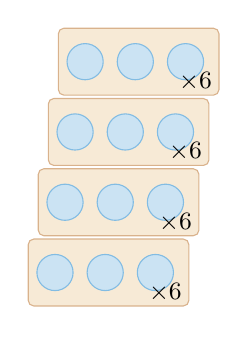
\begin{tikzpicture}[scale=.85]
  \foreach \i in {0,1,2,3}{
    \draw[fill=piasek!80!brown!40,draw=brown!60,rounded corners=2pt] (0.15*\i,\i*1.05) rectangle ++(2.4,1);
    \foreach \j in {0,1,2}{\draw[fill=nieb!25,draw=nieb!60] (0.15*\i+0.4+\j*0.75,\i*1.05+0.5) circle (0.27);}
    \node[font=\sffamily\small\bfseries] at (0.15*\i+2.05,\i*1.05+0.2){$\times 6$};}
\end{tikzpicture}
\end{minipage}\hfill
\begin{minipage}[t]{.6\linewidth}\vspace{0pt}\rmfamily
\cw{A}W sklepie szklanki sprzedaje się tylko w kompletach po 6 sztuk. Ile szklanek kupimy, gdy weźmiemy dwa komplety? A trzy? A cztery?\par\medskip
\sffamily 2 komplety: \ans[1.5cm]\quad 3 komplety: \ans[1.5cm]\quad 4 komplety: \ans[1.5cm]\par\medskip
Jeśli w komplecie jest 6 szklanek, to liczba szklanek, które można kupić, wynosi:\par
\centerline{\large 0,\quad 6,\quad 12,\quad 18,\quad 24,\quad 30,\quad …}
Te liczby nazywamy \textbf{wielokrotnościami} liczby 6.
\end{minipage}

\begin{teoria}
Każda wielokrotność liczby 6 jest wynikiem mnożenia liczby 6 przez jakąś liczbę naturalną:\par
\centerline{0 = 6 · 0,\qquad 6 = 6 · 1,\qquad 12 = 6 · 2,\qquad 18 = 6 · 3,\qquad 24 = 6 · 4,\qquad …}
\end{teoria}

{\rmfamily\cw{B}a) Zapisz kilka wielokrotności liczby 7. \ans[7cm]\par
b) Spośród liczb zakreśl te, które są wielokrotnościami liczby 2:}
\liczby{0,5,14,21,38,150,263}

\begin{uwaga}Zauważ, że liczby parzyste są wielokrotnościami liczby 2, a liczby, które nie są wielokrotnościami liczby 2, są liczbami nieparzystymi.\end{uwaga}

\begin{minipage}[t]{.42\linewidth}\vspace{0pt}
Ola układała zielone paski z jednakowych prostokątów o długości 12 cm, a Wojtek układał czerwone paski z jednakowych prostokątów o długości 14 cm (zobacz rysunek obok).
\end{minipage}\hfill
\begin{minipage}[t]{.55\linewidth}\vspace{0pt}
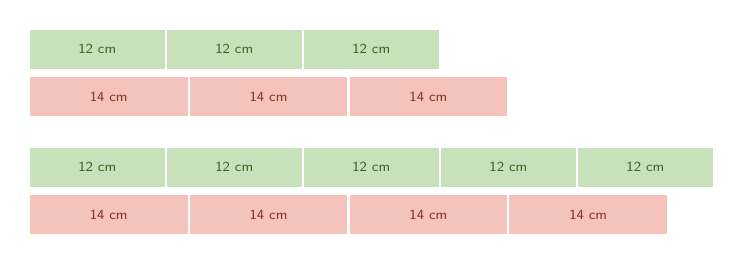
\begin{tikzpicture}[x=1.45mm,y=1mm]
  \newcommand\pasek[4]{\foreach \k in {1,...,#3}{\draw[fill=#4!35,draw=white,line width=.8pt] ({(\k-1)*#2},#1) rectangle ({\k*#2},#1+5.2); \node[font=\sffamily\tiny,text=#4!60!black] at ({(\k-.5)*#2},#1+2.6){#2 cm};}}
  \pasek{21}{12}{3}{ziel}\pasek{15}{14}{3}{czer}\pasek{6}{12}{5}{ziel}\pasek{0}{14}{4}{czer}
\end{tikzpicture}
\end{minipage}

{\rmfamily\cw{C}Jakie długości mają zielone, a jakie czerwone paski na rysunku? Zielone: \ans[1.4cm] cm i \ans[1.4cm] cm, czerwone: \ans[1.4cm] cm i \ans[1.4cm] cm. Jakie inne długości mogą mieć paski ułożone z zielonych prostokątów, a jakie – ułożone z czerwonych?}
\linie{2}

Po kilku próbach Oli i Wojtkowi udało się ułożyć oba paski – zielony i czerwony – tej samej długości. Zastanówmy się, jaką długość mógł mieć każdy z nich.

\clearpage
Długości zielonych pasków wyrażone w centymetrach to wielokrotności liczby 12, a długości czerwonych – wielokrotności liczby 14. Jeśli długość obu pasków ma być taka sama, to musi być zarówno wielokrotnością liczby 12, jak i liczby 14. Musimy więc znaleźć \textbf{wspólną wielokrotność} liczb 12 i 14.

\newcommand\hl[1]{\tikz[baseline=(h.base)]\node[fill=tlozolte,inner sep=1.5pt,rounded corners=1pt](h){#1};}
\begin{minipage}[t]{.55\linewidth}\vspace{0pt}\small
\textbf{Wielokrotności liczby 12:} 0\ \ 12\ \ 24\ \ 36\ \ 48\ \ 60\ \ 72\ \ \hl{84}\ \ 96\ \ 108\ \ 120\ \ 132\ \ 144\ \ 156\ \ \hl{168}\ \ 180\ \ 192\ \ 204\ \ 216\ \ 228\ \ 240\ \ \hl{252}\ \ 264\ \ 276\ \ 288\ \ 300\ \ 312\ \ 324\ \ \hl{336}\par\medskip
\textbf{Wielokrotności liczby 14:} 0\ \ 14\ \ 28\ \ 42\ \ 56\ \ 70\ \ \hl{84}\ \ 98\ \ 112\ \ 126\ \ 140\ \ 154\ \ \hl{168}\ \ 182\ \ 196\ \ 210\ \ 224\ \ 238\ \ \hl{252}\ \ 266\ \ 280\ \ 294\ \ 308\ \ 322\ \ \hl{336}\ \ 350\ \ 364\ \ 378
\end{minipage}\hfill
\begin{minipage}[t]{.41\linewidth}\vspace{0pt}
Zaznaczone liczby: 84, 168, 252, 336 to wspólne, różne od zera wielokrotności liczb 12 i 14. Najmniejszą z nich jest 84. Zapisujemy to w skrócie:\par
\centerline{\large\bfseries NWW(12, 14) = 84}
\centerline{\small Czytamy: najmniejsza wspólna}\centerline{\small wielokrotność liczb 12 i 14 to 84.}
\end{minipage}

\begin{uwaga}\textbf{Uwaga.} Zawsze gdy szukamy najmniejszej wspólnej wielokrotności dwóch liczb różnych od 0, rozważamy tylko wielokrotności różne od 0.\end{uwaga}

{\rmfamily\cw{D}Wypisz kilka wielokrotności liczb 4 i 10. Znajdź NWW(4, 10) = \ans[1.6cm]}
\kratka{1.5}

\zadania
\rmfamily
\nr{1}Podaj kilka przykładów liczb, które są wielokrotnościami:\par
a) liczby 9 \ans[5.5cm]\hfill b) liczby 25 \ans[5.5cm]\par\smallskip
c) liczby 120 \ans[5.3cm]\hfill d) liczby 3000 \ans[5.3cm]

\nr{2}Jakie liczby można wpisać w miejsce kwadracika? \quad \textit{Liczba 18 jest wielokrotnością liczby} \kw\,. \par Wszystkie możliwości: \ans[8cm]

\nr{3}\begin{minipage}[t]{.93\linewidth}Spośród liczb podanych poniżej wypisz te, które są wielokrotnościami liczby:\quad a) 3\qquad b) 8\qquad c) 17
\liczby{0,18,24,34,51,57,72,85,96}
a) \ans[4.5cm]\quad b) \ans[4.5cm]\quad c) \ans[4.5cm]\end{minipage}

\nr{4}a) Znajdź najmniejszą spośród liczb, które są większe od 300 i są wielokrotnościami liczby 40. \ans[1.8cm]\par
b) Znajdź największą spośród liczb, które są mniejsze od 300 i są wielokrotnościami liczby 35. \ans[1.8cm]
\kratka{1.5}

\nr{5}\begin{minipage}[t]{.46\linewidth}a) Liczby $A$, $B$ i $C$ to kolejne wielokrotności liczby 12. Jakie współrzędne mają punkty $A$ i $C$?\par
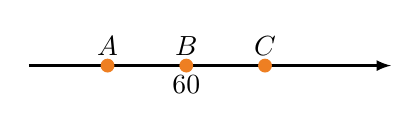
\begin{tikzpicture}[x=1cm]\draw[-latex,thick](0,0)--(4.6,0);\foreach \x/\l in {1/A,2/B,3/C}{\fill[pom](\x,0)circle(2.5pt);\node[above]at(\x,0){$\l$};}\node[below]at(2,0){60};\end{tikzpicture}\par
$A$ = \ans[1.5cm]\quad $C$ = \ans[1.5cm]\end{minipage}\hfill
\begin{minipage}[t]{.46\linewidth}b) Liczby $D$, $E$, $F$ i $G$ to kolejne wielokrotności liczby 9. Jakie współrzędne mają punkty $D$, $F$ i $G$?\par
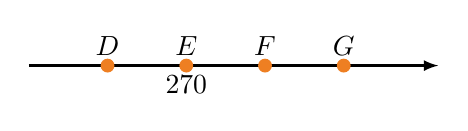
\begin{tikzpicture}[x=1cm]\draw[-latex,thick](0,0)--(5.2,0);\foreach \x/\l in {1/D,2/E,3/F,4/G}{\fill[pom](\x,0)circle(2.5pt);\node[above]at(\x,0){$\l$};}\node[below]at(2,0){270};\end{tikzpicture}\par
$D$ = \ans[1.3cm]\ $F$ = \ans[1.3cm]\ $G$ = \ans[1.3cm]\end{minipage}

\nr{6}\begin{minipage}[t]{.93\linewidth}\tikz\node[draw=pom,line width=1pt,inner sep=5pt,font=\sffamily\small,align=center]{Czterokrotność liczby 15\\to liczba równa 4 · 15.};\par
a) Czterokrotność liczby 15 jest trzykrotnością pewnej liczby. Jaka to liczba? \ans[1.6cm]\par
\gw\ b) Od pięciokrotności pewnej liczby odjęto trzykrotność tej liczby i otrzymano 18. O jakiej liczbie mowa? \ans[1.6cm]\end{minipage}
\kratka{2}

\nr{7}Które z podanych zdań są prawdziwe? Zakreśl P lub F.
\zdanie{1}{Nie ma liczb nieparzystych, które są wielokrotnościami liczby 4.}
\zdanie{2}{Każda liczba parzysta jest wielokrotnością liczby 4.}
\zdanie{3}{Każda liczba naturalna jest wielokrotnością samej siebie.}
\zdanie{4}{Liczba 0 jest wielokrotnością liczby 7.}
\zdanie{5}{Każda wielokrotność liczby 4 jest wielokrotnością liczby 8.}

\nr{8}\gw\ Trzycyfrowa liczba 3\kw 2 jest wielokrotnością liczby 38. Jaką cyfrą należy zastąpić kwadracik? \ans[1.4cm]
\kratka{2}

\nr{9}Podaj NWW (najmniejszą wspólną wielokrotność) liczb:\par\smallskip
\begin{tabular}{@{}llll}
a) 3 i 12 \ans[1.4cm] & c) 4 i 5 \ans[1.4cm] & e) 7 i 13 \ans[1.4cm] & g) 2, 3 i 5 \ans[1.4cm]\\[8pt]
b) 6 i 8 \ans[1.4cm] & d) 1 i 347 \ans[1.4cm] & f) 30 i 15 \ans[1.4cm] & h) 4, 6 i 12 \ans[1.4cm]
\end{tabular}
\kratka{2.5}

\begin{superz}\rmfamily
Ewa i Ola mierzyły stopami długość podwórka. Stopa Ewy ma 25 cm, a stopa Oli – 20 cm. Dziewczynki po każdym postawieniu stopy rysowały kreskę. Nie licząc linii startu, kreska Ewy i kreska Oli 18 razy znalazły się na jednej linii. Czy podwórko ma więcej niż 15 m?
\kratka{2}
Odpowiedź: \ans[6cm]
\end{superz}

% =================== 2. DZIELNIKI ===================
\lekcja{Dzielniki}{Dzielniki}
\begin{minipage}[t]{.36\linewidth}\vspace{0pt}
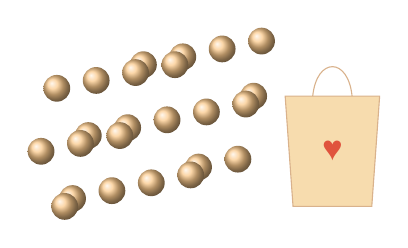
\begin{tikzpicture}
  \foreach \i in {1,...,24}{\pgfmathsetmacro\x{mod(\i*37,30)/10}\pgfmathsetmacro\y{mod(\i*53,22)/10}
    \shade[ball color=pomj!70] (\x,\y) circle (.17);}
  \draw[fill=piasek,draw=brown!60] (3.3,0)--(4.3,0)--(4.4,1.4)--(3.2,1.4)--cycle; \draw[brown!60](3.55,1.4) .. controls (3.6,1.9) and (4,1.9) .. (4.05,1.4);
  \node[text=czer] at (3.8,.7){\ding{170}};
\end{tikzpicture}
\end{minipage}\hfill
\begin{minipage}[t]{.6\linewidth}\vspace{0pt}\rmfamily
\cw{A}a) Mamy 24 cukierki, które chcemy zapakować do torebek po tyle samo sztuk. Po ile cukierków może być w torebkach? \ans[6.5cm]\par\smallskip
b) Po ile cukierków mogłoby się znaleźć w torebkach, gdybyśmy rozdzielali 15 cukierków? \ans[4cm]
\end{minipage}

\medskip
\begin{minipage}[t]{.42\linewidth}\vspace{0pt}
\centering\color{nieb!80!black}\bfseries Mówimy, że dana liczba\\jest podzielna przez jakąś liczbę,\\gdy dzieli się przez nią bez reszty.
\end{minipage}\hfill
\begin{minipage}[t]{.54\linewidth}\vspace{0pt}\rmfamily
\cw{B}Wymień te liczby naturalne, przez które jest podzielna liczba 20. \ans[5cm]
\end{minipage}

\begin{teoria}Każdą liczbę, przez którą liczba 20 jest podzielna, nazywamy jej \textbf{dzielnikiem}. Dzielnikami liczby 20 są: 1, 2, 4, 5, 10 i 20.\end{teoria}

{\rmfamily\cw{C}a) Wypisz wszystkie dzielniki liczby 28. \ans[6cm]\par
b) Ile dzielników ma liczba 1? \ans[1.2cm]\quad Ile dzielników ma liczba 11? \ans[1.2cm]}

\begin{przyklady}
\begin{tabular*}{\linewidth}{@{\extracolsep{\fill}}ccc}
dzielniki liczby 10: & dzielniki liczby 12: & dzielniki liczby 13:\\
1, 2, 5, 10 & 1, 2, 3, 4, 6, 12 & 1, 13
\end{tabular*}
\end{przyklady}

Zauważ, że każda liczba naturalna większa od 1 ma co najmniej dwa dzielniki, bo jest podzielna przez 1 i przez samą siebie.

\begin{minipage}[t]{.44\linewidth}\vspace{0pt}
\begin{tcolorbox}[colback=gray!12,colframe=gray!12,arc=4pt]
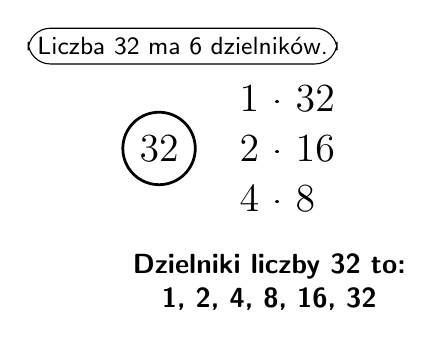
\begin{tikzpicture}
\node[draw=black,line width=1pt,circle,font=\heavy\Large] at (0,0){32};
\node[font=\Large,align=left,anchor=west] at (.9,0){1 · 32\\2 · 16\\4 · 8};
\node[font=\sffamily\bfseries,align=center] at (1.4,-1.7){Dzielniki liczby 32 to:\\1, 2, 4, 8, 16, 32};
\node[draw,rounded corners=8pt,font=\sffamily\small,fill=white] at (0.3,1.3){Liczba 32 ma 6 dzielników.};
\end{tikzpicture}
\end{tcolorbox}
\end{minipage}\hfill
\begin{minipage}[t]{.53\linewidth}\vspace{0pt}
Marta zauważyła, że najłatwiej znaleźć wszystkie dzielniki danej liczby, gdy wypisze się możliwe iloczyny dwóch liczb, które ją dają. Popatrz, jak Marta znalazła dzielniki liczby 32.\par\medskip
{\rmfamily\cw{D}a) Wyjaśnij, na czym polega sposób Marty.\par
b) Znajdź dzielniki liczby 36. \ans[6cm]}
\end{minipage}
\linie{2}

\clearpage
Kartkę o wymiarach 18 cm × 24 cm chcemy pociąć na jednakowe kwadraty o bokach wyrażonych w pełnych centymetrach. Taką kartkę można podzielić na przykład na kwadraty o boku 1 cm, a także na kwadraty o boku 2 cm. Długość boku kwadratów musi być wyrażona liczbą, która jest zarówno dzielnikiem liczby 18, jak i liczby 24. Zatem długość boku największych możliwych kwadratów jest \textbf{największym wspólnym dzielnikiem} tych liczb.

\begin{minipage}[t]{.36\linewidth}\vspace{0pt}
{\color{nieb}\bfseries Dzielniki liczby 18:}\par \hl{1}\ \hl{2}\ \hl{3}\ \hl{6}\ \ 9\ \ 18\par\medskip
{\color{nieb}\bfseries Dzielniki liczby 24:}\par \hl{1}\ \hl{2}\ \hl{3}\ \ 4\ \ \hl{6}\ \ 8\ \ 12\ \ 24
\end{minipage}\hfill
\begin{minipage}[t]{.6\linewidth}\vspace{0pt}
Zaznaczone liczby: 1, 2, 3, 6 to wspólne dzielniki tych liczb. Największym wspólnym dzielnikiem jest 6. Zapisujemy to w skrócie:\par
\centerline{\large\bfseries NWD(18, 24) = 6}
\centerline{\small Czytamy: największy wspólny dzielnik liczb 18 i 24 to 6.}
\end{minipage}

\begin{minipage}[c]{.55\linewidth}
Wobec tego największe kwadraty, na jakie można podzielić kartkę o wymiarach 18 cm × 24 cm, to kwadraty o wymiarach 6 cm × 6 cm.
\end{minipage}\hfill
\begin{minipage}[c]{.4\linewidth}\centering
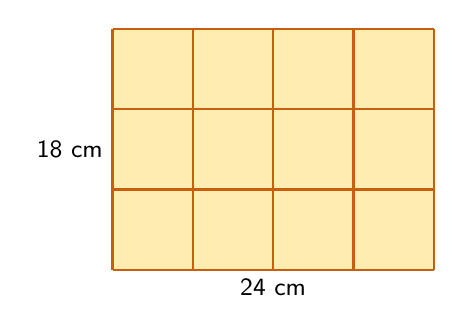
\begin{tikzpicture}[scale=.17]\fill[zolty!45](0,0)rectangle(24,18);\draw[step=6,pomd,line width=.9pt](0,0)grid(24,18);
\node[below,font=\sffamily\small]at(12,0){24 cm};\node[left,font=\sffamily\small]at(0,9){18 cm};\end{tikzpicture}
\end{minipage}

{\rmfamily\cw{E}Znajdź NWD(16, 20). \ans[1.6cm]}
\kratka{1.5}

\zadania\rmfamily
\nr{1}Wypisz wszystkie dzielniki podanej liczby.\par
a) 7 \ans[4.6cm]\hfill b) 8 \ans[4.6cm]\hfill c) 16 \ans[4.6cm]\par\smallskip
d) 27 \ans[4.4cm]\hfill e) 40 \ans[4.6cm]\hfill f) 64 \ans[4.4cm]

\nr{2}Które z podanych zdań są prawdziwe? Zakreśl P lub F.
\zdanie{1}{Liczba 1 jest dzielnikiem każdej liczby naturalnej.}
\zdanie{2}{Liczba 5 jest dzielnikiem każdej liczby, której ostatnią cyfrą jest 0.}
\zdanie{3}{Liczba 2 jest dzielnikiem każdej liczby nieparzystej.}
\zdanie{4}{Każdy dzielnik liczby 12 jest dzielnikiem liczby 36.}
\zdanie{5}{Każdy dzielnik liczby 36 jest dzielnikiem liczby 12.}

\nr{3}Które z podanych liczb są dzielnikami liczby 150? Zakreśl je.
\liczby{1,15,20,30,75,150,300}

\nr{4}\begin{minipage}[t]{.55\linewidth}Do skarbu prowadzą jedne drzwi. Są oznaczone liczbą, dla której suma wszystkich dzielników jest równa 31. Które to drzwi? Zakreśl je.\par\kratka{2}\end{minipage}\hfill
\begin{minipage}[t]{.38\linewidth}\vspace{0pt}\centering
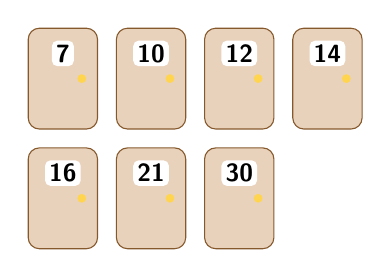
\begin{tikzpicture}[scale=.8]\foreach \n [count=\i] in {7,10,12,14,16,21,30}{\pgfmathsetmacro\x{mod(\i-1,4)*1.4}\pgfmathsetmacro\y{-floor((\i-1)/4)*1.9}
\draw[fill=brown!35,draw=brown!70!black,rounded corners=4pt] (\x,\y) rectangle ++(1.1,1.6);\fill[zolty](\x+.85,\y+.8)circle(.07);\node[fill=white,rounded corners=2pt,inner sep=1.5pt,font=\sffamily\bfseries\small] at (\x+.55,\y+1.2){\n};}\end{tikzpicture}
\end{minipage}

\nr{5}Wypisz wszystkie liczby trzycyfrowe, których dzielnikiem jest:\par
a) 200 \ans[5.5cm]\hfill b) 150 \ans[6cm]\par\smallskip
c) 250 \ans[5.5cm]\hfill d) 300 \ans[6cm]

\nr{6}a) Ile jest liczb trzycyfrowych, których dzielnikiem jest 40? \ans[1.6cm]\par
b) Ile jest liczb czterocyfrowych, których dzielnikiem jest 250? \ans[1.6cm]
\kratka{2}

\begin{minipage}[t]{.44\linewidth}\vspace{0pt}
\begin{ciekawostka}\textbf{Liczba doskonała} to liczba, która jest równa sumie wszystkich swoich dzielników mniejszych od niej. Liczb doskonałych znamy bardzo mało – w 2024 roku znano ich tylko 52.\end{ciekawostka}
\end{minipage}\hfill
\begin{minipage}[t]{.53\linewidth}\vspace{0pt}
\nr{7}Przeczytaj ciekawostkę.\par
a) Wypisz dzielniki liczby 6 mniejsze od 6 i oblicz ich sumę. Czy 6 jest liczbą doskonałą? \opc{tak}\,\opc{nie}\par
b) Czy 28 jest liczbą doskonałą? \opc{tak}\,\opc{nie}\par
c) Czy 12 jest liczbą doskonałą? \opc{tak}\,\opc{nie}
\end{minipage}
\kratka{1.5}

\nr{8}\gw\ Podaj przykład liczby trzycyfrowej, której dzielnikami są liczby 6 i 5. \ans[1.8cm] Znajdź najmniejszą liczbę trzycyfrową, która spełnia te warunki. \ans[1.8cm]

\nr{9}Znajdź NWD (największy wspólny dzielnik) liczb:\par\smallskip
\begin{tabular}{@{}llll}
a) 18 i 30 \ans[1.3cm] & d) 8 i 17 \ans[1.3cm] & g) 27 i 4 \ans[1.3cm] & j) 20 i 300 \ans[1.3cm]\\[8pt]
b) 14 i 15 \ans[1.3cm] & e) 3 i 64 \ans[1.3cm] & h) 13 i 52 \ans[1.3cm] & k) 2 i 777 \ans[1.3cm]\\[8pt]
c) 5 i 20 \ans[1.3cm] & f) 48 i 3 \ans[1.3cm] & i) 9 i 14 \ans[1.3cm] & l) 5 i 405 \ans[1.3cm]
\end{tabular}

\nr{10}Mamy 24 jabłka i 36 gruszek. Chcemy ze wszystkich tych owoców utworzyć jednakowe zestawy jabłek i gruszek. Jaka jest największa możliwa liczba takich zestawów? \ans[1.6cm]
\kratka{1.5}

\nr{11}\gw\ Znajdź wszystkie liczby naturalne większe od 0, ale mniejsze od 30, które można wpisać w miejsce znaku zapytania.\par\smallskip
a) NWD(13, \textcolor{czer}{?}) = 13 \ans[3.5cm]\qquad b) NWD(8, \textcolor{czer}{?}) = 8 \ans[3.5cm]\par\smallskip
c) NWD(\textcolor{czer}{?}, 40) = 5 \ans[3.5cm]\qquad d) NWD(\textcolor{czer}{?}, \textcolor{czer}{?}) = 9 \ (podaj jedną parę) \ans[2.5cm]

\begin{superz}\rmfamily
Pewna liczba ma cztery dzielniki, a ich suma jest równa 32. Jednym z dzielników jest 7. Znajdź tę liczbę.
\kratka{2}
Odpowiedź: \ans[3cm]
\end{superz}

% =================== 3. CECHY ===================
\lekcja{Cechy podzielności liczb}{Cechy podzielności liczb}
{\rmfamily\cw{A}a) Sprawdź, czy liczba 314 jest podzielna przez 4. \opc{tak}\,\opc{nie}\par
b) Sprawdź, czy liczba 1458 jest podzielna przez 9. \opc{tak}\,\opc{nie}}
\kratka{1.5}

Aby ustalić, czy dana liczba jest podzielna przez inną liczbę, można wykonać dzielenie i sprawdzić, czy reszta z dzielenia jest równa 0. Czasami, aby to ustalić, nie trzeba wykonywać dzielenia.

{\rmfamily\cw{B}Spośród liczb podanych na rysunku wypisz:\par
\begin{tabular}{@{}ll}
a) liczby podzielne przez 2, \ans[2.9cm] & c) liczby podzielne przez 10, \ans[2.7cm]\\[8pt]
b) liczby podzielne przez 5, \ans[2.9cm] & d) liczby podzielne przez 100. \ans[2.7cm]
\end{tabular}}

\begin{center}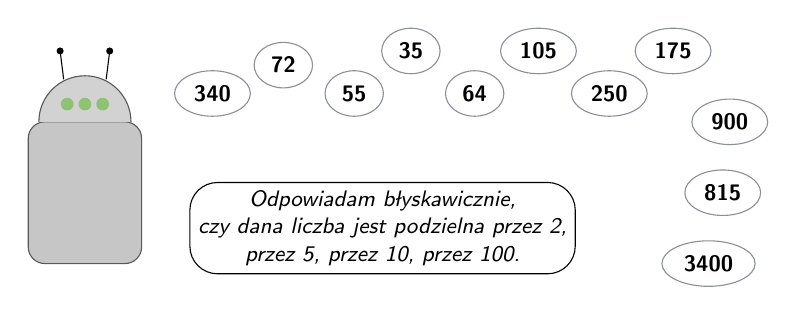
\begin{tikzpicture}[scale=.9,transform shape]
  % robot
  \draw[fill=gray!45,draw=gray!70!black,rounded corners=6pt] (0,0) rectangle (1.6,2);
  \draw[fill=gray!35,draw=gray!70!black] (0.15,2) arc (180:0:.65);
  \foreach \x in {.55,.8,1.05}\fill[ziel!70] (\x,2.25) circle (.09);
  \draw (.5,2.6)--(.45,3)node[circle,fill=black,inner sep=1pt]{}; \draw (1.1,2.6)--(1.15,3)node[circle,fill=black,inner sep=1pt]{};
  \node[draw,rounded corners=10pt,fill=white,font=\sffamily\small\itshape,align=center] at (5,0.5){Odpowiadam błyskawicznie,\\czy dana liczba jest podzielna przez 2,\\przez 5, przez 10, przez 100.};
  \foreach \n/\x/\y in {340/2.6/2.4,72/3.6/2.8,55/4.6/2.4,35/5.4/3.0,64/6.3/2.4,105/7.2/3.0,250/8.2/2.4,175/9.1/3.0,900/9.9/2.0,815/9.8/1.0,3400/9.6/0}
    \node[draw=szary,ellipse,fill=white,font=\sffamily\bfseries\small] at (\x,\y){\n};
\end{tikzpicture}\end{center}

Spróbuj opisać, czym charakteryzują się liczby podzielne przez 10, a czym – liczby podzielne przez 100. Czym charakteryzują się liczby podzielne przez 2, a czym – liczby podzielne przez 5?

Aby rozstrzygnąć, czy liczby są podzielne przez 2, 5, 10 lub 100, można korzystać z poniższych \textbf{cech podzielności liczb}.\par\medskip
\noindent\puzzle{ziel}{Liczba jest podzielna przez 2}{tylko wtedy, gdy jej ostatnią cyfrą jest 0, 2, 4, 6, 8.}{2}\hfill
\puzzle{pom}{Liczba jest podzielna przez 10}{tylko wtedy, gdy jej ostatnią cyfrą jest 0.}{10}\hfill
\puzzle{nieb}{Liczba jest podzielna przez 5}{tylko wtedy, gdy jej ostatnią cyfrą jest 0 lub 5.}{5}\par\medskip
\noindent\puzzle{zolty!80!orange}{Liczba jest podzielna przez 100}{tylko wtedy, gdy jej ostatnie dwie cyfry to 00.}{100}

\clearpage
\begin{minipage}[t]{.42\linewidth}\vspace{0pt}
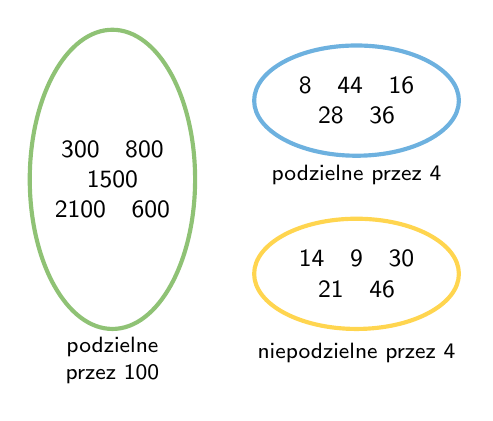
\begin{tikzpicture}[font=\sffamily\small]
  \draw[ziel!70,line width=1.5pt] (0,0) ellipse (1.05 and 1.9);
  \node[align=center] at (0,0){300\quad 800\\1500\\2100\quad 600};
  \node[align=center,font=\sffamily\footnotesize] at (0,-2.3){podzielne\\przez 100};
  \draw[nieb!70,line width=1.5pt] (3.1,1) ellipse (1.3 and .7); \node[align=center] at (3.1,1){8\quad 44\quad 16\\28\quad 36};
  \node[font=\sffamily\footnotesize] at (3.1,0.05){podzielne przez 4};
  \draw[zolty,line width=1.5pt] (3.1,-1.2) ellipse (1.3 and .7); \node[align=center] at (3.1,-1.2){14\quad 9\quad 30\\21\quad 46};
  \node[font=\sffamily\footnotesize] at (3.1,-2.2){niepodzielne przez 4};
\end{tikzpicture}
\end{minipage}\hfill
\begin{minipage}[t]{.54\linewidth}\vspace{0pt}\rmfamily
\cw{C}Przyjrzyj się liczbom w pętlach. Zauważ, że liczby z zielonej pętli także są podzielne przez 4.\par
a) Wybierz jedną liczbę z zielonej pętli i jedną z niebieskiej. Czy ich suma jest podzielna przez 4? \opc{tak}\,\opc{nie}\par
b) Czy można wybrać jedną liczbę z zielonej pętli i jedną z żółtej tak, aby ich suma była podzielna przez 4? \opc{tak}\,\opc{nie}
\end{minipage}

\medskip
\begin{minipage}[t]{.27\linewidth}\vspace{0pt}
\puzzle{ziel}{Liczba jest podzielna przez 4}{tylko wtedy, gdy jej dwie ostatnie cyfry tworzą liczbę podzielną przez 4.}{4}
\end{minipage}\hfill
\begin{minipage}[t]{.68\linewidth}\vspace{0pt}
Wiadomo, że liczba 100 jest podzielna przez 4. Każda liczba naturalna większa od 100 jest sumą wielokrotności liczby 100 i liczby jednocyfrowej lub dwucyfrowej. Podzielność przez 4 zależy więc od dwóch ostatnich cyfr. Opisuje to cecha podzielności podana obok.\par\medskip
{\rmfamily\cw{D}Zapisz każdą z liczb: 436, 1574, 3258, 9612 w postaci sumy wielokrotności liczby 100 i liczby jedno- lub dwucyfrowej. Ustal, które z podanych liczb są podzielne przez 4.}
\end{minipage}
\kratka{2}

{\rmfamily\cw{E}Kuba i Ala zastanawiają się, co można powiedzieć o liczbach podzielnych przez 3. Czy któreś z nich ma rację?}\par
\begin{tikzpicture}
\node[draw,rounded corners=12pt,font=\sffamily\small\itshape,align=center,fill=white] at (0,0){Moim zdaniem każda liczba,\\która jest podzielna przez 3,\\ma ostatnią cyfrę podzielną przez 3.};
\node[font=\sffamily\small] at (0,-1.1){— Kuba};
\node[draw,rounded corners=12pt,font=\sffamily\small\itshape,align=center,fill=white] at (8,0){Ja myślę, że każda liczba\\podzielna przez 3 musi być\\nieparzysta.};
\node[font=\sffamily\small] at (8,-1.1){— Ala};
\end{tikzpicture}
\linie{2}

{\rmfamily\cw{F}Zapisz w zeszycie liczby: 12, 19, 27, 33, 46, 51, 74, 213, 418. Podkreśl na czerwono liczby podzielne przez 3, a na niebiesko – te z liczb, których suma cyfr jest podzielna przez 3.}
\liczby{12,19,27,33,46,51,74,213,418}

\begin{teoria}
Liczby podzielne przez 3 mają wspólną cechę. Suma ich cyfr też jest liczbą podzielną przez 3. Na przykład dla liczb 24, 51, 216, które są podzielne przez 3, otrzymujemy:\par
\begin{center}Suma cyfr liczby 24 to 2 + 4 = 6.\\ Suma cyfr liczby 51 to 5 + 1 = 6.\\ Suma cyfr liczby 216 to 2 + 1 + 6 = 9.\end{center}
Suma cyfr liczb niepodzielnych przez 3 nie jest podzielna przez 3. Na przykład:\par
\begin{center}Suma cyfr liczby 23 to 2 + 3 = 5.\\ Suma cyfr liczby 58 to 5 + 8 = 13.\\ Suma cyfr liczby 151 to 1 + 5 + 1 = 7.\end{center}
\end{teoria}

{\rmfamily\cw{G}Uzupełnij poniższą tabelę, a następnie przyjrzyj się jej uważnie. Co można zauważyć?}\par\smallskip
{\renewcommand{\arraystretch}{1.9}\small
\begin{tabular}{|>{\itshape}l|*{8}{>{\centering\arraybackslash}p{.86cm}|}}\hline
\upshape Liczba & 18 & 36 & 47 & 58 & 702 & 819 & 974 & 4042\\\hline
Czy jest podzielna przez 9? & tak & & & & & & & \\\hline
Ile wynosi suma cyfr? & 9 & & & & & & & \\\hline
Czy suma cyfr jest podzielna przez 9? & tak & & & & & & & \\\hline
\end{tabular}}

\medskip
\noindent\begin{minipage}[t]{.56\linewidth}\vspace{0pt}
\puzzle{nieb}{Liczba jest podzielna przez 3}{tylko wtedy, gdy suma jej cyfr jest liczbą podzielną przez 3.}{3}\ \puzzle{zolty!80!orange}{Liczba jest podzielna przez 9}{tylko wtedy, gdy suma jej cyfr jest liczbą podzielną przez 9.}{9}
\end{minipage}\hfill
\begin{minipage}[t]{.4\linewidth}\vspace{0pt}
Cechy podzielności liczb przez 3 i przez 9 nie przypominają poznanych dotąd cech podzielności. Aby rozstrzygnąć, czy dana liczba jest podzielna przez 3 lub przez 9, musimy najpierw ustalić, ile wynosi suma cyfr tej liczby.
\end{minipage}

\zadania\rmfamily
\nr{1}\begin{minipage}[t]{.93\linewidth}Spośród podanych liczb wypisz liczby podzielne: a) przez 2,\ \ b) przez 5,\ \ c) przez 10,\ \ d) przez 100.
\liczby{20,53,64,85,315,488,730,1250,2006,4700,6205,98\,300,2\,000\,500}
a) \ans[13.5cm]\par\smallskip b) \ans[13.5cm]\par\smallskip c) \ans[13.5cm]\par\smallskip d) \ans[13.5cm]\end{minipage}

\nr{2}Wypisz kilka liczb podzielnych przez 25. \ans[6cm] Czy potrafisz sformułować cechę podzielności przez 25?
\linie{2}

\nr{3}Które z podanych liczb są podzielne przez 4? Zakreśl je.
\liczby{1324,678,516,219,892,63\,514,21\,436}

\nr{4}Asia sprawdzała, czy liczby 1236 oraz 2038 są podzielne przez 4, ale nie korzystała przy tym z cechy podzielności przez 4.\par
\begin{tcolorbox}[colback=gray!10,colframe=gray!10,fontupper=\sffamily\itshape\small,arc=3pt]
\begin{tabular}{@{}l@{\qquad\qquad}l}
1236 – parzysta & 2038 – parzysta\\ 1236 : 2 = 618 – parzysta & 2038 : 2 = 1019 – nieparzysta\\ Liczba 1236 jest podzielna przez 4. & Liczba 2038 nie jest podzielna przez 4.
\end{tabular}\par\smallskip
„Liczba jest podzielna przez 4, gdy jest parzysta i po podzieleniu jej przez 2 otrzymamy liczbę parzystą.”
\end{tcolorbox}
Sprawdź sposobem Asi, które z liczb: 724, 518, 936, 6870, 3354 są podzielne przez 4. \ans[5cm]
\kratka{2}

\begin{ciekawostka}
\begin{multicols}{2}
Obieg Ziemi wokół Słońca trwa 365 dni, 5 godzin, 48 minut i 46 sekund, czyli nieco dłużej niż zwykły rok kalendarzowy, liczący 365 dni. Aby wyrównać tę różnicę, przyjęto, że niektóre lata mają 366 dni. Nazywamy je \textbf{latami przestępnymi}. W takim roku luty jest o 1 dzień dłuższy i ma 29 dni.

Rok jest przestępny, gdy liczba oznaczająca ten rok jest podzielna przez 4. Na przykład latami przestępnymi były 2012, 2016, 2020, 2024, … Od tej reguły jest jednak pewien wyjątek – \textbf{nie są przestępne} lata: 1700, 1800, 1900, 2100, 2200, czyli oznaczone liczbami podzielnymi przez 100, lecz niepodzielnymi przez 400. Za to lata 1600, 2000, 2400 \textbf{są przestępne}.
\end{multicols}
\end{ciekawostka}

\nr{5}Przeczytaj ciekawostkę.\par
a) Czy rok twojego urodzenia był rokiem przestępnym? \opc{tak}\,\opc{nie}\par
b) Czy rok 2026 jest przestępny? \opc{tak}\,\opc{nie}\ \ Podaj dwa najbliższe lata, które będą przestępne. \ans[3cm]\par
c) Które z podanych lat są przestępne? Zakreśl je.
\liczby{1704 r.,1900 r.,1948 r.,1975 r.,2000 r.,2200 r.,2024 r.}
d) Zapisz ostatnie lata wieków: XVIII, XIX i XX. Które z nich to lata przestępne? \ans[5cm]

\nr{6}\begin{minipage}[t]{.62\linewidth}Popatrz na legitymację. Podaj najbliższą od dzisiaj datę, kiedy pani Anna będzie mogła obchodzić rocznicę urodzin w dniu odpowiadającym dacie urodzenia.\par\smallskip \ans[4cm]\end{minipage}\hfill
\begin{minipage}[t]{.3\linewidth}\vspace{0pt}
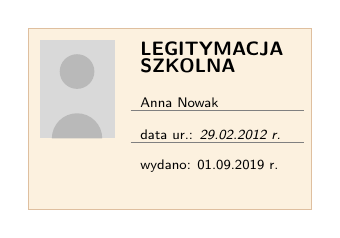
\begin{tikzpicture}[font=\sffamily\tiny]
\draw[fill=piasek!40,draw=brown!50] (0,0) rectangle (3.6,2.3);
\node[anchor=north west,font=\sffamily\scriptsize\bfseries,align=left] at (1.3,2.25){LEGITYMACJA\\[-2pt]SZKOLNA};
\fill[gray!30] (.15,.9) rectangle (1.1,2.15); \fill[gray!55] (.62,1.75) circle (.22); \fill[gray!55] (.3,.9) arc (180:0:.32);
\node[anchor=west] at (1.3,1.35){Anna Nowak};\draw[gray](1.3,1.25)--(3.5,1.25);
\node[anchor=west] at (1.3,.95){data ur.: \itshape 29.02.2012 r.};\draw[gray](1.3,.85)--(3.5,.85);
\node[anchor=west] at (1.3,.55){wydano: 01.09.2019 r.};
\end{tikzpicture}
\end{minipage}

\nr{7}Wśród liczb: 135, 2341, 30\,012, 8127, 41\,022, 1\,000\,001, 56\,789 odszukaj liczby podzielne:\par
a) przez 3 \ans[6cm]\quad b) przez 9 \ans[5cm]
\kratka{1.5}

\nr{8}a) Podaj przykład liczby trzycyfrowej, która jest podzielna przez 3, a nie jest podzielna przez 9. \ans[1.8cm]\par
b) Czy potrafisz podać przykład liczby podzielnej przez 9 i niepodzielnej przez 3? \ans[6cm]

\nr{9}\begin{minipage}[t]{.36\linewidth}\vspace{0pt}
\begin{tcolorbox}[colback=piasek!60,colframe=brown!50,arc=1pt,boxrule=1pt,fontupper=\sffamily\small,halign=center]
{\heavy\large ZAGINĘŁA LICZBA!!!}\par\smallskip
\raggedright Rysopis zaginionej:\par
• jest większa od 7300 i mniejsza od 7400\par • jest podzielna przez 9\par • jest podzielna przez 10\par\smallskip
\centering Uczciwego znalazcę czeka\par{\heavy\Large NAGRODA!}\par\footnotesize Biuro Numerów
\end{tcolorbox}\end{minipage}\hfill
\begin{minipage}[t]{.56\linewidth}\vspace{0pt}
Przeczytaj ogłoszenie zamieszczone obok i ustal, jaka liczba zaginęła w Biurze Numerów. \ans[2cm]\par\medskip
{\color{pom}\heavy\Large 10.}\ Które z podanych sum są podzielne przez 3, a które – przez 9?\par\smallskip
A: 10\textsuperscript{2} + 5\qquad B: 10\textsuperscript{3} + 17\qquad C: 100\textsuperscript{2} + 8\par
D: 10\textsuperscript{3} + 2\qquad E: 100\textsuperscript{3} + 5\par\smallskip
przez 3: \ans[3cm]\quad przez 9: \ans[3cm]
\end{minipage}

\nr{11}Zapisz najmniejszą i największą liczbę dziesięciocyfrową o różnych cyfrach. \ans[3cm]\ \ans[3cm]\par Czy te liczby są podzielne przez 9? \opc{tak}\,\opc{nie}

\nr{12}a) Zapisz kilka liczb trzycyfrowych podzielnych przez 3, używając tylko cyfr 1, 2 lub 3 (cyfry mogą się powtarzać). Ile jest takich liczb? \ans[1.6cm]\par
\gw\ b) Ile jest liczb sześciocyfrowych podzielnych przez 9, zapisanych tylko cyframi 0 lub 3? \ans[1.6cm]
\kratka{2.5}

\nr{13}\begin{minipage}[t]{.6\linewidth}Obok podano klucz do szyfru.\par
a) Jakie słowa zaszyfrowano poniżej?\par
316\quad 201\quad 1205 \ \ans[2.5cm]\par\smallskip
1001\quad 201\quad 1205 \ \ans[2.5cm]\par
b) Utwórz inne słowo z podanych liter i zaszyfruj je liczbami co najmniej trzycyfrowymi.\par\smallskip\ans[6cm]\end{minipage}\hfill
\begin{minipage}[t]{.34\linewidth}\vspace{0pt}
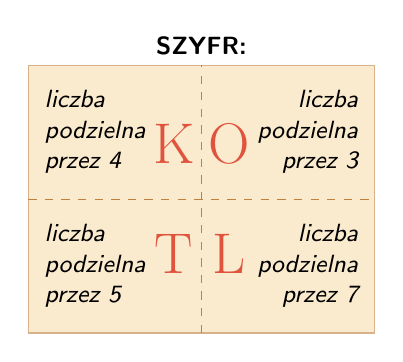
\begin{tikzpicture}[font=\sffamily\small\itshape]
\draw[fill=piasek!60,draw=brown!60] (0,0) rectangle (4.4,3.4);
\draw[dashed,brown] (2.2,0)--(2.2,3.4) (0,1.7)--(4.4,1.7);
\node at (2.2,3.65){\upshape\bfseries SZYFR:};
\node[align=left] at (.85,2.55){liczba\\podzielna\\przez 4}; \node[align=right] at (3.55,2.55){liczba\\podzielna\\przez 3};
\node[align=left] at (.85,.85){liczba\\podzielna\\przez 5}; \node[align=right] at (3.55,.85){liczba\\podzielna\\przez 7};
\node[text=czer,font=\heavy\huge] at (1.85,2.4){K};\node[text=czer,font=\heavy\huge] at (2.55,2.4){O};
\node[text=czer,font=\heavy\huge] at (1.85,1.0){T};\node[text=czer,font=\heavy\huge] at (2.55,1.0){L};
\end{tikzpicture}
\end{minipage}

\nr{14}\gw\ Suma cyfr pewnej wielkiej liczby $a$ wynosi 6456. Czy liczba $a$ jest podzielna przez 3? \opc{tak}\,\opc{nie}\ \ Czy jest podzielna przez 9? \opc{tak}\,\opc{nie}

\nr{15}Zapisz liczby czterocyfrową i pięciocyfrową, takie, że każda z nich:\par
a) jest podzielna przez 5 i przez 4,\ \ans[2cm]\ \ans[2.3cm]\par\smallskip
b) jest podzielna przez 3 i przez 2,\ \ans[2cm]\ \ans[2.3cm]\par\smallskip
c) jest podzielna przez 3 i niepodzielna przez 9.\ \ans[2cm]\ \ans[2.3cm]

\nr{16}a) Podaj przykład liczby trzycyfrowej podzielnej przez 3 i przez 5. \ans[1.8cm] Czy liczba ta jest podzielna przez 15? \opc{tak}\,\opc{nie}\par
b) Sprawdź, nie wykonując dzielenia, czy liczby: 75, 130, 4605, 2253 są podzielne przez 15. \ans[4cm]

\nr{17}\begin{minipage}[t]{.93\linewidth}Korzystając z cech podzielności, wśród liczb podanych niżej odszukaj wielokrotności: a) liczby 6,\ \ b) liczby 12,\ \ c) liczby 20.
\liczby{2460,1356,74\,020,5545,91\,284,403\,101}
a) \ans[4.4cm]\quad b) \ans[4.4cm]\quad c) \ans[4.4cm]\end{minipage}
\kratka{1.5}

\nr{18}Nie wykonując dzielenia, ustal reszty z dzielenia podanych liczb przez 5 oraz reszty z dzielenia przez 4.\par\smallskip
{\renewcommand{\arraystretch}{1.9}
\begin{tabular}{|l|*{5}{>{\centering\arraybackslash}p{1.5cm}|}}\hline
liczba & 2437 & 8104 & 5326 & 9999 & 6750\\\hline
reszta z dzielenia przez 5 & & & & & \\\hline
reszta z dzielenia przez 4 & & & & & \\\hline
\end{tabular}}

\nr{19}\gw\ a) Nie wykonując dzielenia, znajdź reszty z dzielenia przez 3 liczb: 715 \ans[1.2cm], 6023 \ans[1.2cm], 88\,011 \ans[1.2cm].\par
b) Zapisz dziewięć kolejnych liczb trzycyfrowych. Nie wykonując dzielenia, znajdź reszty z dzielenia tych liczb przez 9.
\kratka{2}

\begin{superz}\rmfamily
\begin{minipage}[t]{.7\linewidth}Jaką cyfrą należy zastąpić znak \romb, aby otrzymać liczbę, której resztą z dzielenia przez 12 jest 2?\end{minipage}\hfill{\heavy\LARGE 25\romb 8}
\kratka{2}
Odpowiedź: \ans[2cm]
\end{superz}

% =================== 4. PIERWSZE ===================
\lekcja{Liczby pierwsze i liczby złożone}{Liczby pierwsze i liczby złożone}
{\rmfamily\cw{A}Zapisz, ile dzielników ma każda z liczb: 6 \ans[1.1cm],\ 7 \ans[1.1cm],\ 15 \ans[1.1cm],\ 17 \ans[1.1cm].}

Każda liczba naturalna większa od 1 ma co najmniej dwa dzielniki, gdyż jest podzielna przez 1 i przez samą siebie.

{\rmfamily\cw{B}Podaj trzy przykłady liczb, które mają:\par
a) więcej niż dwa dzielniki, \ans[4cm]\qquad b) tylko dwa dzielniki. \ans[4cm]}

\begin{teoria}
Liczbę naturalną, która ma dokładnie dwa dzielniki, nazywamy \textbf{liczbą pierwszą}. Przykłady liczb pierwszych:\par
\centerline{2, 3, 5, 7, 11, 13, 17, 19, 23}
Liczbę naturalną różną od zera, która ma więcej niż dwa dzielniki, nazywamy \textbf{liczbą złożoną}. Przykłady liczb złożonych:\par
\centerline{4, 6, 8, 9, 10, 12, 14, 15, 16}
Liczby 0 i 1 nie są ani pierwsze, ani złożone.
\end{teoria}

\textbf{Sito Eratostenesa.} Skreśl liczbę 1. Zakreśl kółkiem 2 i skreśl wszystkie jej wielokrotności. Potem zakreśl 3 i skreśl jej wielokrotności, następnie 5 i 7. Liczby, które zostaną, to liczby pierwsze mniejsze od 100.\par\smallskip
\begin{center}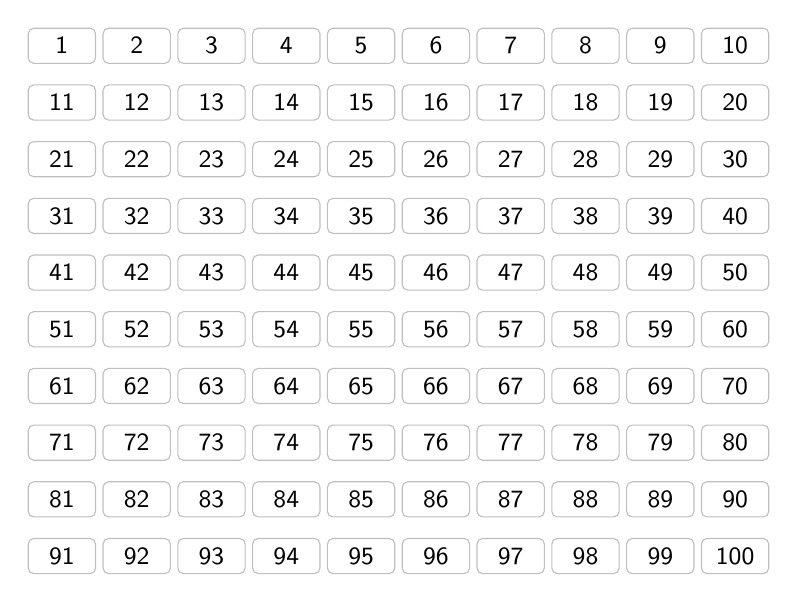
\begin{tikzpicture}[x=.95cm,y=.72cm]
\foreach \k in {1,...,100}{\pgfmathtruncatemacro\i{mod(\k-1,10)}\pgfmathtruncatemacro\j{floor((\k-1)/10)}
 \draw[gray!50,fill=white,rounded corners=2pt] (\i,-\j) rectangle ++(.9,.62); \node[font=\sffamily\small] at (\i+.45,-\j+.31){\k};}
\end{tikzpicture}\end{center}
Ile liczb pierwszych mniejszych od 100 znalazłeś? \ans[1.6cm]

\begin{ciekawostka}
\begin{multicols}{2}
Liczb pierwszych jest nieskończenie wiele. Znajdowanie ich nie jest jednak łatwe. Od pewnego czasu używa się do tego komputerów i dzięki temu co jakiś czas są odkrywane coraz większe liczby pierwsze.

Na przykład w 2024 roku odkryto za pomocą komputerów kolejną ogromną liczbę pierwszą, która ma aż 41\,024\,320 cyfr. Gdyby cyfry tej liczby zapisać jedna za drugą na pasku papieru, to miałby on długość około 164 km.
\end{multicols}
\end{ciekawostka}

\clearpage
\zadania\rmfamily
\nr{1}Uzasadnij, że liczby: 2316, 4785, 1818, 2721, 7413 są złożone (dla każdej z nich znajdź dzielnik różny od 1 i różny od tej liczby; możesz skorzystać z cech podzielności liczb).\par\smallskip
2316: \ans[1.3cm]\quad 4785: \ans[1.3cm]\quad 1818: \ans[1.3cm]\quad 2721: \ans[1.3cm]\quad 7413: \ans[1.3cm]

\nr{2}\begin{minipage}[t]{.5\linewidth}\vspace{0pt}
\begin{tcolorbox}[colback=zolty!25,colframe=zolty!25,arc=2pt,left=2pt,right=2pt,top=2pt,bottom=2pt,fontupper=\sffamily\scriptsize]
\setlength{\tabcolsep}{2.2pt}\begin{tabular}{*{8}{r}}2 & 3 & 5 & 7 & 11 & 13 & 17 & 19\\
23 & 29 & 31 & 37 & 41 & 43 & 47 & 53\\
59 & 61 & 67 & 71 & 73 & 79 & 83 & 89\\
97 & 101 & 103 & 107 & 109 & 113 & 127 & 131\\
137 & 139 & 149 & 151 & 157 & 163 & 167 & 173\\
179 & 181 & 191 & 193 & 197 & 199 & 211 & 223\\
227 & 229 & 233 & 239 & 241 & 251 & 257 & 263\\
269 & 271 & 277 & 281 & 283 & 293 & 307 & 311\\
313 & 317 & 331 & 337 & 347 & 349 & 353 & 359\\
367 & 373 & 379 & 383 & 389 & 397 & 401 & 409\\
419 & 421 & 431 & 433 & 439 & 443 & 449 & 457\\
461 & 463 & 467 & 479 & 487 & 491 & 499 & 503\\
509 & 521 & 523 & 541 & 547 & 557 & 563 & 569\\
571 & 577 & 587 & 593 & 599 & 601 & 607 & 613\\
617 & 619 & 631 & 641 & 643 & 647 & 653 & 659\\
661 & 673 & 677 & 683 & 691 & 701 & 709 & 719\\
727 & 733 & 739 & 743 & 751 & 757 & 761 & 769\\
773 & 787 & 797 & 809 & 811 & 821 & 823 & 827\\
829 & 839 & 853 & 857 & 859 & 863 & 877 & 881\\
883 & 887 & 907 & 911 & 919 & 929 & 937 & 941\\
947 & 953 & 967 & 971 & 977 & 983 & 991 & 997\end{tabular}
\end{tcolorbox}
\end{minipage}\hfill
\begin{minipage}[t]{.45\linewidth}\vspace{0pt}
Obok zamieszczono wszystkie liczby pierwsze mniejsze od 1000. Odpowiedz na pytania:\par\smallskip
a) Jaka jest najmniejsza trzycyfrowa liczba pierwsza, a jaka największa?\par \ans[1.6cm]\ \ans[1.6cm]\par\smallskip
b) Ile jest liczb pierwszych mniejszych od 1000? \ans[1.6cm]\par\smallskip
c) Ile jest liczb złożonych mniejszych od 1000? \ans[1.6cm]
\kratka{2}
{\color{pom}\heavy\Large 3.}\ a) Liczba 2003 jest liczbą pierwszą. Wypisz jej dzielniki. \ans[3cm]\par\smallskip
b) Jakie cyfry na pewno nie mogą być cyframi jedności liczby pierwszej większej od 10? \ans[4cm]
\end{minipage}

\nr{4}Które z podanych zdań są prawdziwe? Zakreśl P lub F.
\zdanie{1}{Każda liczba parzysta większa od 2 jest złożona.}
\zdanie{2}{Iloczyn dwóch liczb pierwszych jest liczbą złożoną.}
\zdanie{3}{Liczba 1 jest najmniejszą liczbą pierwszą.}
\zdanie{4}{Suma dwóch nieparzystych liczb pierwszych jest liczbą pierwszą.}
\zdanie{5}{Liczba 2 jest jedyną parzystą liczbą pierwszą.}

\nr{5}Liczba 31 jest liczbą pierwszą. Znajdź NWD(100, 31). \ans[1.6cm]

\nr{6}\gw\ Wśród dziewięciu liczb podanych obok są cztery liczby pierwsze. Które to liczby? Zakreśl je.
\liczby{5371,111\,111,103,6981,70\,707,827,1993,42\,983,2027}
\kratka{2}

\begin{superz}\rmfamily
Ile dzielników ma kwadrat liczby pierwszej (np. 7 · 7)? \ans[1.6cm]\par
A ile dzielników ma trzecia potęga liczby pierwszej (np. 2 · 2 · 2)? \ans[1.6cm]
\kratka{1.5}
\end{superz}

% =================== 5. ROZKŁAD ===================
\lekcja{Rozkład na czynniki pierwsze}{Rozkład na czynniki pierwsze}
{\small\color{szary}Lekcja dodatkowa – w podręczniku „Matematyka z kluczem” (Nowa Era) dla klasy 5 ten temat występuje zaraz po liczbach pierwszych i złożonych.}

\begin{teoria}
Każdą liczbę złożoną można zapisać w postaci iloczynu liczb pierwszych. Taki zapis nazywamy \textbf{rozkładem liczby na czynniki pierwsze}.\par
Na przykład:\quad 60 = 2 · 2 · 3 · 5,\qquad 84 = 2 · 2 · 3 · 7,\qquad 45 = 3 · 3 · 5.
\end{teoria}

\begin{minipage}[t]{.55\linewidth}\vspace{0pt}
\textbf{Jak rozkładamy liczbę?} Zapisujemy liczbę i stawiamy obok pionową kreskę. Dzielimy przez najmniejszą liczbę pierwszą, przez którą się da (2, 3, 5, 7, …). Wynik zapisujemy pod spodem. Powtarzamy, aż otrzymamy 1.\par\medskip
\textbf{NWD i NWW z rozkładu} (24 i 36):\par
24 = \hl{2 · 2} · 2 · \hl{3}\qquad 36 = \hl{2 · 2} · \hl{3} · 3\par
NWD = iloczyn wspólnych czynników = 2 · 2 · 3 = 12\par
NWW = 2 · 2 · 2 · 3 · 3 = 72
\end{minipage}\hfill
\begin{minipage}[t]{.38\linewidth}\vspace{0pt}\centering
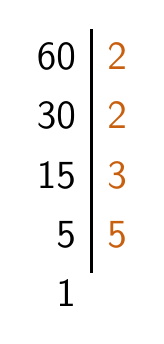
\begin{tikzpicture}[font=\sffamily\Large]
\foreach \a/\b [count=\i] in {60/2,30/2,15/3,5/5,1/}{\node[anchor=east] at (0,-\i*.75){\a};\node[anchor=west,text=pomd] at (.15,-\i*.75){\b};}
\draw[line width=1.2pt] (0.07,-.4)--(0.07,-3.5);
\end{tikzpicture}\par
{\large 60 = 2 · 2 · 3 · 5}
\end{minipage}

\zadania\rmfamily
\nr{1}Rozłóż liczby na czynniki pierwsze.\par
\begin{tabular}{@{}lll}
18 = \ans[3.2cm] & 45 = \ans[3.2cm] & 72 = \ans[3.2cm]\\[8pt]
100 = \ans[3.2cm] & 126 = \ans[3.2cm] & 210 = \ans[3.2cm]
\end{tabular}
\kratka{3.5}

\nr{2}Jaka liczba ma rozkład:\quad a) 2 · 3 · 3 · 5 \ans[1.5cm]\quad b) 2 · 2 · 2 · 7 \ans[1.5cm]\quad c) 3 · 5 · 11 \ans[1.5cm]

\nr{3}Korzystając z rozkładu na czynniki pierwsze, oblicz:\par
NWD(12, 18) = \ans[1.4cm]\quad NWW(12, 18) = \ans[1.4cm]\quad NWD(30, 45) = \ans[1.4cm]\quad NWW(30, 45) = \ans[1.4cm]
\kratka{3}

\nr{4}\gw\ Uzupełnij rozkład:\quad 168 = 2 · 2 · 2 · \kw\ · 7\qquad 330 = 2 · \kw\ · 5 · 11

% =================== SPRAWDZIANY ===================
\lekcja{Sprawdziany}{Sprawdzian 1: Wielokrotności}
Imię i nazwisko: \ans[7cm]\hfill Data: \ans[3cm]\par\smallskip
{\small\color{szary}Za każde zadanie 1 punkt (razem 10 pkt). Wynik wpisz w ramkę, a obliczenia zapisz w kratkach. W zadaniach z wyborem zakreśl jedną odpowiedź.}\par
\nr{1}{\rmfamily Trzycyfrowa liczba \textbf{9\kw{}2} jest wielokrotnością liczby 26. Jaką cyfrę trzeba wpisać w okienko?}\par
\kratka{1.5}\hfill Odpowiedź: \ans[2.8cm]\par
\nr{2}{\rmfamily Oblicz \textbf{NWW(6, 5, 10)}.}\par
\kratka{1.5}\hfill Odpowiedź: \ans[2.8cm]\par
\nr{3}{\rmfamily Oblicz \textbf{NWW(6, 15)}.}\par
\kratka{1.5}\hfill Odpowiedź: \ans[2.8cm]\par
\nr{4}{\rmfamily Dziewięciokrotność liczby 14 jest dwukrotnością pewnej liczby. Jaka to liczba?}\par
\kratka{1.5}\hfill Odpowiedź: \ans[2.8cm]\par
\nr{5}{\rmfamily Liczby A, B, C to \textbf{kolejne} wielokrotności liczby 9. B = 90. Ile wynosi A?}\par
\kratka{1.5}\hfill Odpowiedź: \ans[2.8cm]\par
\nr{6}{\rmfamily Prawda czy fałsz? \\ \textit{„Każda wielokrotność liczby 4 jest wielokrotnością liczby 2.”}}\par
\smallskip \opc{A. Prawda}\quad \opc{B. Fałsz}\par
\nr{7}{\rmfamily Która z liczb jest wielokrotnością liczby \textbf{12}?}\par
\smallskip \opc{A. 160}\quad \opc{B. 161}\quad \opc{C. 171}\quad \opc{D. 156}\par
\kratka{1}
\nr{8}{\rmfamily Znajdź \textbf{największą} liczbę mniejszą od 162, która jest wielokrotnością liczby 45.}\par
\kratka{1.5}\hfill Odpowiedź: \ans[2.8cm]\par
\nr{9}{\rmfamily Od czterokrotności pewnej liczby odjęto dwukrotność tej liczby i otrzymano 4. O jakiej liczbie mowa?}\par
\kratka{1.5}\hfill Odpowiedź: \ans[2.8cm]\par
\nr{10}{\rmfamily Znajdź \textbf{najmniejszą} liczbę większą od 135, która jest wielokrotnością liczby 50.}\par
\kratka{1.5}\hfill Odpowiedź: \ans[2.8cm]\par
\par\bigskip\begin{tcolorbox}[colback=krem,colframe=pom!40,arc=6pt,fontupper=\sffamily\small]Punkty: \ans[1.5cm] / 10\hfill Ocena: \ans[3cm]\par\smallskip Skala: 0–29\% – 1,\ 30–49\% – 2,\ 50–69\% – 3,\ 70–84\% – 4,\ 85–95\% – 5,\ 96–100\% – 6.\end{tcolorbox}
\lekcja{Sprawdziany}{Sprawdzian 2: Dzielniki}
Imię i nazwisko: \ans[7cm]\hfill Data: \ans[3cm]\par\smallskip
{\small\color{szary}Za każde zadanie 1 punkt (razem 10 pkt). Wynik wpisz w ramkę, a obliczenia zapisz w kratkach. W zadaniach z wyborem zakreśl jedną odpowiedź.}\par
\nr{1}{\rmfamily Ile dzielników ma liczba \textbf{28}?}\par
\kratka{1.5}\hfill Odpowiedź: \ans[2.8cm]\par
\nr{2}{\rmfamily Znajdź najmniejszą liczbę \textbf{trzycyfrową}, której dzielnikami są liczby 12 i 5.}\par
\kratka{1.5}\hfill Odpowiedź: \ans[2.8cm]\par
\nr{3}{\rmfamily Kartkę 36 cm × 45 cm tniemy na jednakowe kwadraty o boku w pełnych centymetrach (bez odpadów). Jaki najdłuższy bok (w cm) mogą mieć kwadraty?}\par
\kratka{1.5}\hfill Odpowiedź: \ans[2.8cm]\par
\nr{4}{\rmfamily Która liczba \textbf{NIE} jest dzielnikiem liczby 30?}\par
\smallskip \opc{A. 16}\quad \opc{B. 15}\quad \opc{C. 6}\quad \opc{D. 5}\par
\kratka{1}
\nr{5}{\rmfamily Mamy 48 niebieskich kredek i 60 czerwonych kredek. Chcemy ze \textbf{wszystkich} ułożyć jednakowe zestawy. Ile najwięcej zestawów można ułożyć?}\par
\kratka{1.5}\hfill Odpowiedź: \ans[2.8cm]\par
\nr{6}{\rmfamily Oblicz sumę \textbf{wszystkich} dzielników liczby 14.}\par
\kratka{1.5}\hfill Odpowiedź: \ans[2.8cm]\par
\nr{7}{\rmfamily Oblicz \textbf{NWD(15, 35)}.}\par
\kratka{1.5}\hfill Odpowiedź: \ans[2.8cm]\par
\nr{8}{\rmfamily Prawda czy fałsz? \\ \textit{„Każdy dzielnik liczby 12 jest dzielnikiem liczby 24.”}}\par
\smallskip \opc{A. Prawda}\quad \opc{B. Fałsz}\par
\nr{9}{\rmfamily Ile jest liczb \textbf{trzycyfrowych}, których dzielnikiem jest 150?}\par
\kratka{1.5}\hfill Odpowiedź: \ans[2.8cm]\par
\nr{10}{\rmfamily \textbf{Liczba doskonała} jest równa sumie swoich dzielników mniejszych od niej. Czy 12 jest liczbą doskonałą?}\par
\smallskip \opc{A. Tak}\quad \opc{B. Nie}\par
\par\bigskip\begin{tcolorbox}[colback=krem,colframe=pom!40,arc=6pt,fontupper=\sffamily\small]Punkty: \ans[1.5cm] / 10\hfill Ocena: \ans[3cm]\par\smallskip Skala: 0–29\% – 1,\ 30–49\% – 2,\ 50–69\% – 3,\ 70–84\% – 4,\ 85–95\% – 5,\ 96–100\% – 6.\end{tcolorbox}
\lekcja{Sprawdziany}{Sprawdzian 3: Cechy podzielności}
Imię i nazwisko: \ans[7cm]\hfill Data: \ans[3cm]\par\smallskip
{\small\color{szary}Za każde zadanie 1 punkt (razem 10 pkt). Wynik wpisz w ramkę, a obliczenia zapisz w kratkach. W zadaniach z wyborem zakreśl jedną odpowiedź.}\par
\nr{1}{\rmfamily Czy rok \textbf{1850} jest przestępny?}\par
\smallskip \opc{A. Tak}\quad \opc{B. Nie}\par
\nr{2}{\rmfamily Zaginęła liczba! Jest większa od 9400 i mniejsza od 9500, dzieli się przez 9 i przez 10. Jaka to liczba?}\par
\kratka{1.5}\hfill Odpowiedź: \ans[2.8cm]\par
\nr{3}{\rmfamily Która liczba jest podzielna przez \textbf{15}?}\par
\smallskip \opc{A. 4200}\quad \opc{B. 8103}\quad \opc{C. 3823}\quad \opc{D. 1898}\par
\kratka{1}
\nr{4}{\rmfamily Nie wykonując dzielenia, podaj resztę z dzielenia liczby \textbf{26\,646} przez 5.}\par
\kratka{1.5}\hfill Odpowiedź: \ans[2.8cm]\par
\nr{5}{\rmfamily Prawda czy fałsz? \\ \textit{„Każda liczba podzielna przez 3 jest nieparzysta.”}}\par
\smallskip \opc{A. Prawda}\quad \opc{B. Fałsz}\par
\nr{6}{\rmfamily Jaką cyfrę trzeba wpisać w okienko, żeby liczba \textbf{9\kw{}04} była podzielna przez 9?}\par
\kratka{1.5}\hfill Odpowiedź: \ans[2.8cm]\par
\nr{7}{\rmfamily Suma cyfr pewnej liczby wynosi \textbf{2160}. Czy ta liczba jest podzielna przez 9?}\par
\smallskip \opc{A. Tak}\quad \opc{B. Nie}\par
\nr{8}{\rmfamily Jaką \textbf{najmniejszą} cyfrę można wpisać w okienko, żeby liczba \textbf{5\kw{}3} była podzielna przez 3?}\par
\kratka{1.5}\hfill Odpowiedź: \ans[2.8cm]\par
\nr{9}{\rmfamily Która liczba jest podzielna przez \textbf{10}?}\par
\smallskip \opc{A. 25\,500}\quad \opc{B. 25\,487}\quad \opc{C. 74\,408}\quad \opc{D. 98\,618}\par
\kratka{1}
\nr{10}{\rmfamily Która liczba jest podzielna przez \textbf{6}?}\par
\smallskip \opc{A. 5794}\quad \opc{B. 1306}\quad \opc{C. 2526}\quad \opc{D. 2158}\par
\kratka{1}
\par\bigskip\begin{tcolorbox}[colback=krem,colframe=pom!40,arc=6pt,fontupper=\sffamily\small]Punkty: \ans[1.5cm] / 10\hfill Ocena: \ans[3cm]\par\smallskip Skala: 0–29\% – 1,\ 30–49\% – 2,\ 50–69\% – 3,\ 70–84\% – 4,\ 85–95\% – 5,\ 96–100\% – 6.\end{tcolorbox}
\lekcja{Sprawdziany}{Sprawdzian 4: Liczby pierwsze}
Imię i nazwisko: \ans[7cm]\hfill Data: \ans[3cm]\par\smallskip
{\small\color{szary}Za każde zadanie 1 punkt (razem 10 pkt). Wynik wpisz w ramkę, a obliczenia zapisz w kratkach. W zadaniach z wyborem zakreśl jedną odpowiedź.}\par
\nr{1}{\rmfamily Którą cyfrą jedności \textbf{nie może} kończyć się liczba pierwsza większa od 10?}\par
\smallskip \opc{A. 7}\quad \opc{B. 1}\quad \opc{C. 6}\quad \opc{D. 3}\par
\kratka{1}
\nr{2}{\rmfamily Prawda czy fałsz? \\ \textit{„Liczba 2 jest jedyną parzystą liczbą pierwszą.”}}\par
\smallskip \opc{A. Prawda}\quad \opc{B. Fałsz}\par
\nr{3}{\rmfamily Podaj dowolny dzielnik liczby \textbf{221} różny od 1 i od 221 (to pokazuje, że jest złożona).}\par
\kratka{1.5}\hfill Odpowiedź: \ans[2.8cm]\par
\nr{4}{\rmfamily Jaka jest najmniejsza liczba pierwsza \textbf{większa} od 82?}\par
\kratka{1.5}\hfill Odpowiedź: \ans[2.8cm]\par
\nr{5}{\rmfamily Liczba 59 jest pierwsza. Oblicz \textbf{NWD(61, 59)}.}\par
\kratka{1.5}\hfill Odpowiedź: \ans[2.8cm]\par
\nr{6}{\rmfamily Która z liczb jest \textbf{pierwsza}?}\par
\smallskip \opc{A. 69}\quad \opc{B. 117}\quad \opc{C. 83}\quad \opc{D. 147}\par
\kratka{1}
\nr{7}{\rmfamily Ile jest liczb pierwszych większych od 30 i mniejszych od 60?}\par
\kratka{1.5}\hfill Odpowiedź: \ans[2.8cm]\par
\nr{8}{\rmfamily Która z liczb jest \textbf{złożona}?}\par
\smallskip \opc{A. 113}\quad \opc{B. 101}\quad \opc{C. 37}\quad \opc{D. 121}\par
\kratka{1}
\nr{9}{\rmfamily Ile dzielników ma liczba \textbf{49} (7 · 7)?}\par
\kratka{1.5}\hfill Odpowiedź: \ans[2.8cm]\par
\nr{10}{\rmfamily Ile jest liczb pierwszych większych od 40 i mniejszych od 60?}\par
\kratka{1.5}\hfill Odpowiedź: \ans[2.8cm]\par
\par\bigskip\begin{tcolorbox}[colback=krem,colframe=pom!40,arc=6pt,fontupper=\sffamily\small]Punkty: \ans[1.5cm] / 10\hfill Ocena: \ans[3cm]\par\smallskip Skala: 0–29\% – 1,\ 30–49\% – 2,\ 50–69\% – 3,\ 70–84\% – 4,\ 85–95\% – 5,\ 96–100\% – 6.\end{tcolorbox}
\lekcja{Sprawdziany}{Sprawdzian 5: Rozkład na czynniki}
Imię i nazwisko: \ans[7cm]\hfill Data: \ans[3cm]\par\smallskip
{\small\color{szary}Za każde zadanie 1 punkt (razem 8 pkt). Wynik wpisz w ramkę, a obliczenia zapisz w kratkach. W zadaniach z wyborem zakreśl jedną odpowiedź.}\par
\nr{1}{\rmfamily Jaka liczba ma rozkład na czynniki pierwsze \textbf{2 · 2 · 5}?}\par
\kratka{1.5}\hfill Odpowiedź: \ans[2.8cm]\par
\nr{2}{\rmfamily Jaki jest \textbf{największy} czynnik pierwszy liczby 384?}\par
\kratka{1.5}\hfill Odpowiedź: \ans[2.8cm]\par
\nr{3}{\rmfamily Uzupełnij rozkład: \textbf{45 = 3 · \kw{} · 5}}\par
\kratka{1.5}\hfill Odpowiedź: \ans[2.8cm]\par
\nr{4}{\rmfamily Ile czynników (licząc powtórzenia) ma rozkład liczby \textbf{298} na czynniki pierwsze?}\par
\kratka{1.5}\hfill Odpowiedź: \ans[2.8cm]\par
\nr{5}{\rmfamily 20 = 2 · 2 · 5, ~ 9 = 3 · 3. Oblicz \textbf{NWW(20, 9)}.}\par
\kratka{1.5}\hfill Odpowiedź: \ans[2.8cm]\par
\nr{6}{\rmfamily 8 = 2 · 2 · 2, ~ 20 = 2 · 2 · 5. Oblicz \textbf{NWD(8, 20)}.}\par
\kratka{1.5}\hfill Odpowiedź: \ans[2.8cm]\par
\nr{7}{\rmfamily 18 = 2 · 3 · 3, ~ 15 = 3 · 5. Oblicz \textbf{NWW(18, 15)}.}\par
\kratka{1.5}\hfill Odpowiedź: \ans[2.8cm]\par
\nr{8}{\rmfamily 42 = 2 · 3 · 7, ~ 18 = 2 · 3 · 3. Oblicz \textbf{NWD(42, 18)}.}\par
\kratka{1.5}\hfill Odpowiedź: \ans[2.8cm]\par
\par\bigskip\begin{tcolorbox}[colback=krem,colframe=pom!40,arc=6pt,fontupper=\sffamily\small]Punkty: \ans[1.5cm] / 8\hfill Ocena: \ans[3cm]\par\smallskip Skala: 0–29\% – 1,\ 30–49\% – 2,\ 50–69\% – 3,\ 70–84\% – 4,\ 85–95\% – 5,\ 96–100\% – 6.\end{tcolorbox}
\lekcja{Sprawdziany}{Sprawdzian zbiorczy}
Imię i nazwisko: \ans[7cm]\hfill Data: \ans[3cm]\par\smallskip
{\small\color{szary}Za każde zadanie 1 punkt (razem 16 pkt). Wynik wpisz w ramkę, a obliczenia zapisz w kratkach. W zadaniach z wyborem zakreśl jedną odpowiedź.}\par
\nr{1}{\rmfamily Liczba 23 jest pierwsza. Oblicz \textbf{NWD(191, 23)}.}\par
\kratka{1.5}\hfill Odpowiedź: \ans[2.8cm]\par
\nr{2}{\rmfamily Nie wykonując dzielenia, podaj resztę z dzielenia liczby \textbf{27\,918} przez 9.}\par
\kratka{1.5}\hfill Odpowiedź: \ans[2.8cm]\par
\nr{3}{\rmfamily Suma cyfr pewnej liczby wynosi \textbf{9186}. Czy ta liczba jest podzielna przez 3?}\par
\smallskip \opc{A. Tak}\quad \opc{B. Nie}\par
\nr{4}{\rmfamily Oblicz \textbf{NWW(5, 8, 10)}.}\par
\kratka{1.5}\hfill Odpowiedź: \ans[2.8cm]\par
\nr{5}{\rmfamily Mamy 18 cukierków i 24 lizaków. Chcemy ze \textbf{wszystkich} ułożyć jednakowe zestawy. Ile najwięcej zestawów można ułożyć?}\par
\kratka{1.5}\hfill Odpowiedź: \ans[2.8cm]\par
\nr{6}{\rmfamily Znajdź \textbf{największą} liczbę mniejszą od 632, która jest wielokrotnością liczby 80.}\par
\kratka{1.5}\hfill Odpowiedź: \ans[2.8cm]\par
\nr{7}{\rmfamily Która liczba \textbf{NIE} jest dzielnikiem liczby 40?}\par
\smallskip \opc{A. 20}\quad \opc{B. 10}\quad \opc{C. 2}\quad \opc{D. 22}\par
\kratka{1}
\nr{8}{\rmfamily Która liczba jest podzielna przez \textbf{2}?}\par
\smallskip \opc{A. 83\,067}\quad \opc{B. 56\,537}\quad \opc{C. 41\,775}\quad \opc{D. 42\,446}\par
\kratka{1}
\nr{9}{\rmfamily Prawda czy fałsz? \\ \textit{„Liczba 13 ma dokładnie dwa dzielniki.”}}\par
\smallskip \opc{A. Prawda}\quad \opc{B. Fałsz}\par
\nr{10}{\rmfamily Uzupełnij rozkład: \textbf{56 = \kw{} · 2 · 2 · 7}}\par
\kratka{1.5}\hfill Odpowiedź: \ans[2.8cm]\par
\nr{11}{\rmfamily Od pięciokrotności pewnej liczby odjęto trzykrotność tej liczby i otrzymano 26. O jakiej liczbie mowa?}\par
\kratka{1.5}\hfill Odpowiedź: \ans[2.8cm]\par
\nr{12}{\rmfamily Jaka jest najmniejsza liczba pierwsza \textbf{większa} od 39?}\par
\kratka{1.5}\hfill Odpowiedź: \ans[2.8cm]\par
\nr{13}{\rmfamily \textbf{Liczba doskonała} jest równa sumie swoich dzielników mniejszych od niej. Czy 18 jest liczbą doskonałą?}\par
\smallskip \opc{A. Tak}\quad \opc{B. Nie}\par
\nr{14}{\rmfamily Ile czynników (licząc powtórzenia) ma rozkład liczby \textbf{228} na czynniki pierwsze?}\par
\kratka{1.5}\hfill Odpowiedź: \ans[2.8cm]\par
\nr{15}{\rmfamily Znajdź \textbf{najmniejszą} liczbę większą od 381, która jest wielokrotnością liczby 40.}\par
\kratka{1.5}\hfill Odpowiedź: \ans[2.8cm]\par
\nr{16}{\rmfamily Która z liczb jest \textbf{złożona}?}\par
\smallskip \opc{A. 109}\quad \opc{B. 59}\quad \opc{C. 169}\quad \opc{D. 29}\par
\kratka{1}
\par\bigskip\begin{tcolorbox}[colback=krem,colframe=pom!40,arc=6pt,fontupper=\sffamily\small]Punkty: \ans[1.5cm] / 16\hfill Ocena: \ans[3cm]\par\smallskip Skala: 0–29\% – 1,\ 30–49\% – 2,\ 50–69\% – 3,\ 70–84\% – 4,\ 85–95\% – 5,\ 96–100\% – 6.\end{tcolorbox}

% =================== ODPOWIEDZI ===================
\lekcja{Odpowiedzi}{Odpowiedzi}
\small\sffamily
\begin{multicols}{2}
\newcommand\odp[1]{\par\smallskip{\color{pomd}\bfseries #1}\par}
\odp{1. Wielokrotności}
Ćw. A: 12, 18, 24. Ćw. B: a) np. 0, 7, 14, 21, 28; b) 0, 14, 38, 150. Ćw. C: zielone 36 i 60 cm, czerwone 42 i 56 cm; inne – wielokrotności 12 i 14. Ćw. D: NWW(4, 10) = 20.\par
1. np. a) 9, 18, 27 b) 25, 50, 75 c) 120, 240, 360 d) 3000, 6000, 9000.
2. 1, 2, 3, 6, 9, 18.
3. a) 0, 18, 24, 51, 57, 72, 96 b) 0, 24, 72, 96 c) 0, 34, 51, 85.
4. a) 320 b) 280.
5. a) A = 48, C = 72 b) D = 261, F = 279, G = 288.
6. a) 20 b) 9.
7. P, F, P, P, F.
8. 4 (342 = 38 · 9).
9. a) 12 b) 24 c) 20 d) 347 e) 91 f) 30 g) 30 h) 12.\par
Super zagadka: kreski spotykają się co NWW(25, 20) = 100 cm, więc podwórko ma co najmniej 18 m – tak.

\odp{2. Dzielniki}
Ćw. A: a) 1, 2, 3, 4, 6, 8, 12, 24 b) 1, 3, 5, 15. Ćw. B: 1, 2, 4, 5, 10, 20. Ćw. C: a) 1, 2, 4, 7, 14, 28 b) 1; 2. Ćw. D: b) 1, 2, 3, 4, 6, 9, 12, 18, 36. Ćw. E: 4.\par
1. a) 1, 7 b) 1, 2, 4, 8 c) 1, 2, 4, 8, 16 d) 1, 3, 9, 27 e) 1, 2, 4, 5, 8, 10, 20, 40 f) 1, 2, 4, 8, 16, 32, 64.
2. P, P, F, P, F.
3. 1, 15, 30, 75, 150.
4. Drzwi 16 (1 + 2 + 4 + 8 + 16 = 31).
5. a) 200, 400, 600, 800 b) 150, 300, 450, 600, 750, 900 c) 250, 500, 750 d) 300, 600, 900.
6. a) 22 b) 36.
7. a) 1 + 2 + 3 = 6 – tak b) tak (1 + 2 + 4 + 7 + 14 = 28) c) nie (1 + 2 + 3 + 4 + 6 = 16).
8. np. 150; najmniejsza 120.
9. a) 6 b) 1 c) 5 d) 1 e) 1 f) 3 g) 1 h) 13 i) 1 j) 20 k) 1 l) 5.
10. 12 zestawów (po 2 jabłka i 3 gruszki).
11. a) 13, 26 b) 8, 16, 24 c) 5, 15, 25 d) np. 9 i 18, 9 i 27, 18 i 27.\par
Super zagadka: 21 (1 + 3 + 7 + 21 = 32).

\odp{3. Cechy podzielności}
Ćw. A: a) nie b) tak. Ćw. B: a) 340, 72, 64, 250, 900, 3400 b) 340, 55, 35, 105, 250, 175, 900, 815, 3400 c) 340, 250, 900, 3400 d) 900, 3400. Ćw. C: a) tak b) nie. Ćw. D: 436 i 9612. Ćw. E: nikt (np. 12). Ćw. F: 12, 27, 33, 51, 213 (obie grupy takie same). Ćw. G: 36 – tak, 9, tak; 47 – nie, 11, nie; 58 – nie, 13, nie; 702 – tak, 9, tak; 819 – tak, 18, tak; 974 – nie, 20, nie; 4042 – nie, 10, nie.\par
1. a) 20, 64, 488, 730, 1250, 2006, 4700, 98\,300, 2\,000\,500 b) 20, 85, 315, 730, 1250, 4700, 6205, 98\,300, 2\,000\,500 c) 20, 730, 1250, 4700, 98\,300, 2\,000\,500 d) 4700, 98\,300, 2\,000\,500.
2. Dwie ostatnie cyfry: 00, 25, 50 lub 75.
3. 1324, 516, 892, 21\,436.
4. 724, 936.
5. b) nie; 2028 i 2032 c) 1704, 1948, 2000, 2024 d) 1800, 1900, 2000 – przestępny tylko 2000.
6. 29 lutego 2028 r.
7. a) 135, 30\,012, 8127, 41\,022 b) 135, 8127, 41\,022.
8. a) np. 123 b) nie.
9. 7380.
10. przez 3: A, B, C, D, E; przez 9: B, C.
11. 1\,023\,456\,789 i 9\,876\,543\,210 – tak (suma cyfr 45).
12. a) 9 b) 11.
13. a) KOT, LOT.
14. tak; nie.
15. np. a) 1020, 10\,020 b) 1002, 10\,002 c) 1002, 10\,002.
16. a) np. 105 – tak b) 75 i 4605.
17. a) 2460, 1356, 91\,284 b) 2460, 1356, 91\,284 c) 2460, 74\,020.
18. przez 5: 2, 4, 1, 4, 0; przez 4: 1, 0, 2, 3, 2.
19. a) 1, 2, 0.\par
Super zagadka: 5 (2558 = 12 · 213 + 2).

\odp{4. Liczby pierwsze i złożone}
Ćw. A: 4, 2, 4, 2. Sito: 25 liczb.\par
1. np. 2316 – 2, 4785 – 5, 1818 – 2, 2721 – 3, 7413 – 3.
2. a) 101 i 997 b) 168 c) 830.
3. a) 1, 2003 b) 0, 2, 4, 5, 6, 8.
4. P, P, F, F, P.
5. 1.
6. 103, 827, 1993, 2027.\par
Super zagadka: 3; 4.

\odp{5. Rozkład na czynniki}
1. 18 = 2 · 3 · 3; 45 = 3 · 3 · 5; 72 = 2 · 2 · 2 · 3 · 3; 100 = 2 · 2 · 5 · 5; 126 = 2 · 3 · 3 · 7; 210 = 2 · 3 · 5 · 7.
2. a) 90 b) 56 c) 165.
3. 6; 36; 15; 90.
4. 3; 3.

\textbf{\large Sprawdziany}\par\smallskip
\textbf{\color{pomd}Sprawdzian 1: Wielokrotności}\par
1. 6 {\color{szary}– 962 = 26 · 37.}\par
2. 30 {\color{szary}– 30 to najmniejsza liczba (różna od 0), która dzieli się przez 6, 5, 10.}\par
3. 30 {\color{szary}– Wypisujemy wielokrotności większej liczby: 15, 30 – pierwsza, która dzieli się przez 6, to \textbf{30}.}\par
4. 63 {\color{szary}– 9 · 14 = 126, a 126 : 2 = 63.}\par
5. 81 {\color{szary}– Kolejne wielokrotności liczby 9 różnią się o 9: A = 81, B = 90, C = 99.}\par
6. A. Prawda {\color{szary}– 4 · n = 2 · (2 · n).}\par
7. D. 156 {\color{szary}– 156 = 12 · 13. Pozostałe liczby nie dzielą się przez 12 bez reszty.}\par
8. 135 {\color{szary}– 135 = 45 · 3; następna wielokrotność 180 jest już $\geq$ 162.}\par
9. 2 {\color{szary}– 4 · x − 2 · x = 2 · x = 4, więc x = 4 : 2 = 2.}\par
10. 150 {\color{szary}– 150 = 50 · 3, a poprzednia wielokrotność 100 nie jest większa od 135.}\par
\medskip
\textbf{\color{pomd}Sprawdzian 2: Dzielniki}\par
1. 6 {\color{szary}– Dzielniki 28: 1, 2, 4, 7, 14, 28 – razem 6.}\par
2. 120 {\color{szary}– Musi to być wielokrotność NWW(12, 5) = 60. Najmniejsza trzycyfrowa: 120.}\par
3. 9 {\color{szary}– Bok musi dzielić 36 i 45: NWD = 9.}\par
4. A. 16 {\color{szary}– 30 : 16 daje resztę 14. Dzielniki 30: 1, 2, 3, 5, 6, 10, 15, 30.}\par
5. 12 {\color{szary}– Liczba zestawów musi dzielić 48 i 60: NWD(48, 60) = 12.}\par
6. 24 {\color{szary}– 1 + 2 + 7 + 14 = 24.}\par
7. 5 {\color{szary}– Wspólne dzielniki 15 i 35: 1, 5. Największy to 5.}\par
8. A. Prawda {\color{szary}– 24 = 2 · 12, więc co dzieli 12, dzieli też 24.}\par
9. 6 {\color{szary}– Pierwsza: 150, ostatnia: 900. To wielokrotności 150 od 1. do 6. – razem 6.}\par
10. B. Nie {\color{szary}– 1 + 2 + 3 + 4 + 6 = 16 $\neq$ 12.}\par
\medskip
\textbf{\color{pomd}Sprawdzian 3: Cechy podzielności}\par
1. B. Nie {\color{szary}– 1850 nie dzieli się przez 4 (dwie ostatnie cyfry: 50).}\par
2. 9450 {\color{szary}– Dzieli się przez 10, więc kończy się zerem; suma cyfr ma dzielić się przez 9: 9450 (suma 18).}\par
3. A. 4200 {\color{szary}– Liczba dzieli się przez 15, gdy dzieli się przez 3 i przez 5. 4200 = 15 · 280.}\par
4. 1 {\color{szary}– Reszta = 1, bo ostatnia cyfra 6.}\par
5. B. Fałsz {\color{szary}– Np. 6 jest parzysta.}\par
6. 5 {\color{szary}– Suma pozostałych cyfr to 13. Dopełniamy do wielokrotności 9: brakuje 5.}\par
7. A. Tak {\color{szary}– Wystarczy sprawdzić sumę cyfr: 2160 dzieli się przez 9 (suma jej cyfr: 9).}\par
8. 1 {\color{szary}– Suma pozostałych cyfr: 8. Najmniejsza cyfra, która dopełnia do wielokrotności 3, to 1.}\par
9. A. 25\,500 {\color{szary}– Cecha podzielności przez 10: ostatnia cyfra 0. 25\,500 ją spełnia.}\par
10. C. 2526 {\color{szary}– Liczba dzieli się przez 6, gdy dzieli się przez 2 i przez 3. 2526 = 6 · 421.}\par
\medskip
\textbf{\color{pomd}Sprawdzian 4: Liczby pierwsze}\par
1. C. 6 {\color{szary}– Liczba kończąca się na 6 dzieli się przez 2, więc jest złożona.}\par
2. A. Prawda {\color{szary}– Inne parzyste dzielą się przez 2.}\par
3. np. 13 {\color{szary}– Np. 13: 221 = 13 · 17.}\par
4. 83 {\color{szary}– Sprawdzamy kolejne liczby po 82: pierwszą liczbą pierwszą jest 83.}\par
5. 1 {\color{szary}– 59 ma dzielniki tylko 1 i 59, a 61 nie dzieli się przez 59, więc NWD = 1.}\par
6. C. 83 {\color{szary}– 83 ma tylko dwa dzielniki: 1 i 83. Pozostałe są złożone.}\par
7. 7 {\color{szary}– To: 31, 37, 41, 43, 47, 53, 59.}\par
8. D. 121 {\color{szary}– 121 = 11 · 11, więc ma więcej niż dwa dzielniki.}\par
9. 3 {\color{szary}– Dzielniki: 1, 7, 49 – razem 3.}\par
10. 5 {\color{szary}– To: 41, 43, 47, 53, 59.}\par
\medskip
\textbf{\color{pomd}Sprawdzian 5: Rozkład na czynniki}\par
1. 20 {\color{szary}– 2 · 2 · 5 = 20.}\par
2. 3 {\color{szary}– 384 = 2 · 2 · 2 · 2 · 2 · 2 · 2 · 3.}\par
3. 3 {\color{szary}– 45 = 3 · 3 · 5.}\par
4. 2 {\color{szary}– 298 = 2 · 149 – 2 czynniki.}\par
5. 180 {\color{szary}– NWW = 2 · 2 · 3 · 3 · 5 = 180.}\par
6. 4 {\color{szary}– Wspólne czynniki: 2 · 2 = 4.}\par
7. 90 {\color{szary}– NWW = 2 · 3 · 3 · 5 = 90.}\par
8. 6 {\color{szary}– Wspólne czynniki: 2 · 3 = 6.}\par
\medskip
\textbf{\color{pomd}Sprawdzian zbiorczy}\par
1. 1 {\color{szary}– 23 ma dzielniki tylko 1 i 23, a 191 nie dzieli się przez 23, więc NWD = 1.}\par
2. 0 {\color{szary}– Reszta = 0, bo suma cyfr 27 daje z dzielenia przez 9 resztę 0.}\par
3. A. Tak {\color{szary}– Wystarczy sprawdzić sumę cyfr: 9186 dzieli się przez 3 (suma jej cyfr: 24).}\par
4. 40 {\color{szary}– 40 to najmniejsza liczba (różna od 0), która dzieli się przez 5, 8, 10.}\par
5. 6 {\color{szary}– Liczba zestawów musi dzielić 18 i 24: NWD(18, 24) = 6.}\par
6. 560 {\color{szary}– 560 = 80 · 7; następna wielokrotność 640 jest już $\geq$ 632.}\par
7. D. 22 {\color{szary}– 40 : 22 daje resztę 18. Dzielniki 40: 1, 2, 4, 5, 8, 10, 20, 40.}\par
8. D. 42\,446 {\color{szary}– Cecha podzielności przez 2: ostatnia cyfra 0, 2, 4, 6 lub 8. 42\,446 ją spełnia.}\par
9. A. Prawda {\color{szary}– 1 i 13.}\par
10. 2 {\color{szary}– 56 = 2 · 2 · 2 · 7.}\par
11. 13 {\color{szary}– 5 · x − 3 · x = 2 · x = 26, więc x = 26 : 2 = 13.}\par
12. 41 {\color{szary}– Sprawdzamy kolejne liczby po 39: pierwszą liczbą pierwszą jest 41.}\par
13. B. Nie {\color{szary}– 1 + 2 + 3 + 6 + 9 = 21 $\neq$ 18.}\par
14. 4 {\color{szary}– 228 = 2 · 2 · 3 · 19 – 4 czynniki.}\par
15. 400 {\color{szary}– 400 = 40 · 10, a poprzednia wielokrotność 360 nie jest większa od 381.}\par
16. C. 169 {\color{szary}– 169 = 13 · 13, więc ma więcej niż dwa dzielniki.}\par
\medskip
\end{multicols}
\end{document}
